% 附录 B 微分形式的一些应用
\chapter{微分形式的一些应用}

在本附录中, 我们将试着宽泛地展示数学与物理中一些使用微分形式的领域. 在读完一本关于微分形式的这么厚的书之后, 读者应该对除电磁学之外的一些应用有所了解, 这会很好. 这些小节的任何一个都无意接近完备. 相反, 它们旨在开阔读者的眼界, 对每个主题只给一点点尝味, 并希望能勾起读者进一步探究的欲望.

第 1 节以非常一般的方式介绍 de Rham 上同调. 在某种意义上, 这是微分形式的一个"硬核"数学应用. 基本上, 微分形式可以用来研究流形的拓扑. 在第 2 节我们考察几个 de Rham 上同调群的例子, 看看它们如何被用来了解流形的整体拓扑. 第 3 节引入辛流形的思想, 以及最常见的辛流形——任意流形的余切丛. 辛流形引出辛几何. 第 4 节介绍 Darboux 定理, 它是辛几何的一个基本结果. 然后第 5 节讨论辛几何的一个物理应用, 即几何力学.

\section{de Rham 上同调引论}

在下一节中, 我们将对一个名为 de Rham 上同调的数学分支给出非常简短的介绍. 本质上, de Rham 上同调在流形 $M$ 上的微分形式与该流形的整体拓扑之间建立联系. 这是一个不可思议且内容丰富的数学领域, 我们所能做的不会超过给出一个入门性的浏览. 我们将使用微分形式, 特别是闭形式与恰当形式之间的关系, 来确定流形的整体拓扑信息. 这基本上让我们能够利用本质上是微积分式的计算来确定整体拓扑性质. 但这里"整体"与"拓扑"这两个词是什么意思？我们不会尝试给出严格的定义, 但会试着让你对它们的含义有一种感觉.

你可以大致把拓扑想成对流形、或 $\mathbb{R}^n$ 的子集如何连通、以及该流形或子集有多少个"洞"的研究. 而我们说的流形的"整体"性质（相对于局部性质）是什么意思？回忆我们对流形的直观想法：它是局部欧几里得的东西. 更精确一点, 一个 $n$ 维流形被相互重叠的坐标片 $U_i$ 覆盖, 其中 $U_i$ 是映射 $\varphi_i:\mathbb{R}^n\to U_i$ 的像. 例如, 在图~\ref{fig:B-1} 中, 流形 $M=\mathbb{R}^2-\{(0,0)\}$（即缺少原点的平面）画有四个坐标片. 每个点 $p\in M$ 都包含在某个与 $\mathbb{R}^2$ 的开邻域本质上相同的开邻域中.

\begin{figure}[htbp]
  \centering
  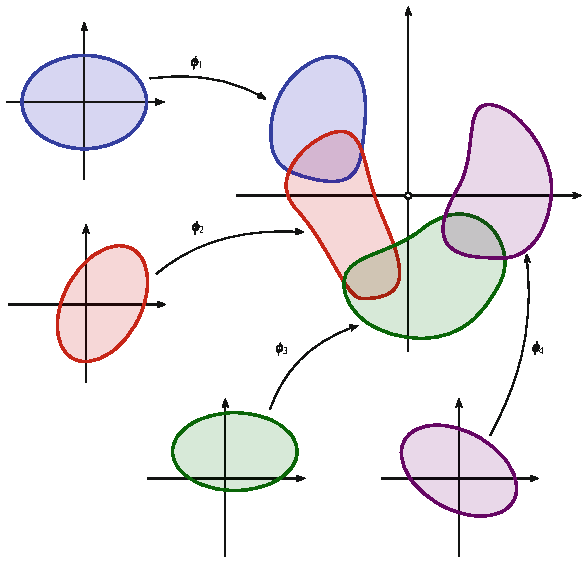
\includegraphics[width=0.960\linewidth]{images/vector/fig-B-1.pdf}
  \caption{带四个坐标片的流形 $M=\mathbb{R}^2-\{(0,0)\}$}
  \label{fig:B-1}
\end{figure}

所以 $M=\mathbb{R}^2-\{(0,0)\}$ 的局部信息与 $\mathbb{R}^2$ 中的局部信息相同. 但显然在 $M$ 中我们缺少了一个点, 即原点. 由于只缺少一个点, 你可能会受到诱惑, 用"局部"一词的通常用法去认为缺少的点是局部性质, 但它不是. 缺少原点实际上是一个整体性质；它说明了关于整个流形的某些东西, 即该流形有一个洞. $M$ 有一个洞这一事实是一个整体拓扑性质.

我们可以使用定义在流形上的某些微分形式来探测像洞这样的整体性质. 在探测整体性质时, 某些形式是有趣的, 某些形式则一点也不有趣. 事实证明, 有趣的形式是那些外微分为零的形式, 即闭形式.

\begin{figure}[htbp]
  \centering
  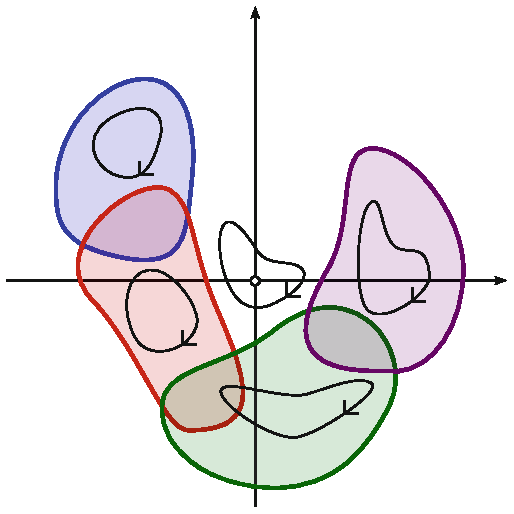
\includegraphics[width=0.711\linewidth]{images/vector/fig-B-2.pdf}
  \caption{流形 $M=\mathbb{R}^2-\{(0,0)\}$ 画有五个小的闭曲线. 其中四个曲线包含在单个坐标片内, 而第五个曲线围住原点处的洞. 这条曲线不能完全画在单个坐标片内}
  \label{fig:B-2}
\end{figure}

暂时我们把"闭形式给出整体信息"的说法放在一边, 而是试着向你说明闭形式不给出局部信息. 假设 $\alpha$ 是闭形式. 在 $M$ 上局部地看, 即在某个坐标片 $U_i$ 内部, 我们在某个完全位于坐标片 $U_i$ 内部的小闭曲线 $C$ 上积分 $\alpha$；也就是在一条"局部"曲线上积分. 见图~\ref{fig:B-2}.

\begin{figure}[htbp]
  \centering
  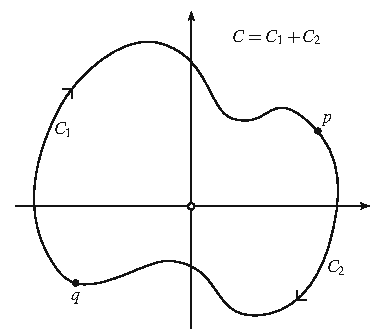
\includegraphics[width=0.452\linewidth]{images/vector/fig-B-3.pdf}
  \caption{被分成两条曲线 $C_1$ 与 $C_2$ 的闭曲线 $C$, $C=C_1+C_2$}
  \label{fig:B-3}
\end{figure}

对位于单个坐标片内部、因而是某个区域 $D$ 的边界的局部曲线 $C$ 使用 Stokes 定理, 我们有
\[
\oint_{C=\partial D}\alpha=\int_D d\alpha=\int_D 0=0.
\]
由于 $\alpha$ 在局部曲线上的积分为零, 这告诉我们在流形局部什么也没有. 所以闭形式不给我们任何关于流形的局部信息. 当然, 到现在你也许已经猜到闭形式有趣的"整体"本质如何产生了. 如果我们沿着一条围绕原点处缺失点的曲线积分一个闭的 $\alpha$ 会怎么样？首先, 这条曲线不再完全包含在单个坐标片 $U_i$ 中. 如果我们有 $\oint_C\alpha\neq0$, 那么我们就知道对某个区域 $D$ 有 $C\neq\partial D$, 并且曲线 $C$ 内部一定有什么奇怪的事情发生. 存在一条曲线 $C$ 使得闭的 $\alpha$ 满足 $\oint_C\alpha\neq0$ 这一事实本身, 就告诉了我们关于 $M$ 的某些整体拓扑信息. 如果 $C$ 不是某个区域 $D$ 的边界, 那么 $C$ 必然围住某种洞.

现在假设 $\alpha$ 是恰当的, 即存在 $\beta$ 使得 $\alpha=d\beta$. 我们将会看到恰当形式不是有趣的. 对任意闭曲线 $C$, 无论 $C$ 是否围住洞, 通过在曲线 $C$ 上选取两个点 $p$ 与 $q$, 我们可以把曲线分成两部分：从 $q$ 到 $p$ 的 $C_1$ 和从 $p$ 到 $q$ 的 $C_2$, 如图~\ref{fig:B-3} 所示. 现在 $C$ 由两条曲线 $C_1$ 与 $C_2$ 一起组成. 我们常写 $C=C_1+C_2$. 于是有
\[
\begin{aligned}
\oint_C\alpha&=\int_{C_1+C_2}\alpha\\
&=\int_{C_1}\alpha+\int_{C_2}\alpha\\
&=\int_{C_1}d\beta+\int_{C_2}d\beta\\
&=\int_{\partial C_1}\beta+\int_{\partial C_2}\beta\\
&=\int_{\{p\}-\{q\}}\beta+\int_{\{q\}-\{p\}}\beta\\
&=\int_{\{p\}-\{q\}}\beta-\int_{\{p\}-\{q\}}\beta\\
&=0.
\end{aligned}
\]
换言之, 对恰当形式 $\alpha$, 无论 $C$ 是否围住洞, 我们都有 $\oint_C\alpha=0$. 换句话说, 恰当形式不是有趣的, 至少在告诉我们关于洞的某些东西这方面不是.

如果我们所处的情形是流形为 $\mathbb{R}^n$, 那么由 Poincaré 引理, 每个闭形式都是恰当的. 这意味着闭形式的集合与恰当形式的集合相同, 于是不存在曲线 $C$ 使得对闭的 $\alpha$ 有 $\oint_C\alpha\neq0$. 但这不应太让我们吃惊, 因为我们知道 $\mathbb{R}^n$ 中没有任何洞.

我们基本上感兴趣的是闭形式的集合与恰当形式的集合不同的情形. 我们想要某种方式来度量这两个集合有多大差别. 在图~\ref{fig:B-4} 中, 我们用类似维恩图的图画来帮助可视化这一情形.

\begin{figure}[htbp]
  \centering
  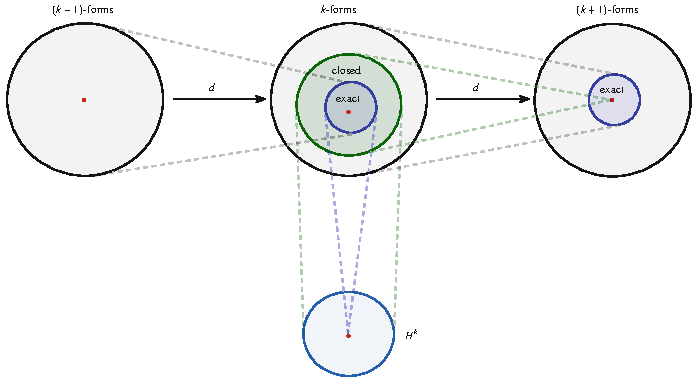
\includegraphics[width=0.960\linewidth]{images/vector/fig-B-4.pdf}
  \caption{我们希望度量闭 $k$-形式的集合与恰当 $k$-形式的集合有多大差别. 我们通过等价类 $H_{\mathrm{dR}}^k(M)$ 做到这一点（Bachman~\cite{ref04}, 2006, p.118）}
  \label{fig:B-4}
\end{figure}

我们感兴趣的是以某种方式度量一组闭形式离恰当有多远. 我们通过所谓的\newterm{equivalence-relation}{等价关系}{equivalence relation}做到这一点. 等价关系就是：取一组对象, 通过在原集合中定义某些对象"相同"来创造另一组对象的一种方式. 事实上, 我们在第 10.2 节用曲线的等价类定义切向量时已经见识过这个概念的实际运作. 在那里, 如果满足某些判据, 我们就定义两条曲线等价, 或者说"相同". 这里, 流形 $M$ 上的两个闭 $k$-形式 $\alpha$ 与 $\beta$, 如果它们的差是恰当的, 就被认为是相同或等价的. 换言之, 如果 $\alpha-\beta$ 是 $M$ 上的恰当 $k$-形式, 我们就认为 $\alpha$ 与 $\beta$ 等价. 更精确地说, 假设 $\alpha$ 与 $\beta$ 是 $M$ 上的两个闭 $k$-形式. 那么如果对某个 $(k-1)$-形式 $\omega$ 有
\[
\alpha-\beta=d\omega,
\]
我们就说 $\alpha$ 等价于 $\beta$, 记为 $\alpha\sim\beta$. 我们把 $\alpha$ 的等价类记为
\[
[\alpha]=\left\{\beta\in\Omega^k(M)\;\middle|\;\alpha\sim\beta\right\}.
\]
当我们这样做时, 我们最终得到一个集合, 其元素是相差一个恰当形式的闭形式的等价类. 这个集合记为 $H_{\mathrm{dR}}^k(M)$：
\[
H_{\mathrm{dR}}^k(M)=\frac{\left\{\alpha\in\Omega^k(M)\;\middle|\;d\alpha=0\right\}}{\left\{d\omega\in\Omega^k(M)\;\middle|\;\omega\in\Omega^{k-1}(M)\right\}}.
\]
大声朗读时, 中间的横线读作 modulo, 或简称 mod. 右边会被读作"闭形式模恰当形式". 这个 $H_{\mathrm{dR}}^k(M)$ 称为第 $k$ 个 de Rham 上同调群. 这个向量空间 $H_{\mathrm{dR}}^k(M)$ 实际上在告诉我们关于流形 $M$ 的连通性和洞的个数的某些东西.

我们不会在本书中解释 group（群）这个词是什么意思, 但如果你还没有上过抽象代数课, 请注意 group 一词在数学中有非常精确的含义, 不能轻率或不精确地使用. 不幸的是, 或者也许是幸运的是, 对我们来说, de Rham 上同调群实际上也是一个向量空间, 后者在第 1.1 节定义过. 事实证明, 向量空间确实是定义了标量乘法的交换群. 也就是说, 向量空间是在其上定义了某些附加结构的交换群；附加结构就是标量乘法. 标量乘法只不过意味着你可以用标量乘空间中的元素, 标量不过是实数 $c\in\mathbb{R}$ 的另一个说法. 所以, 把 de Rham 上同调群称为群虽然并非不准确, 但也不是尽可能准确. de Rham 上同调群是一个向量空间. 但正如语言中常发生的那样, 一旦一个名字被附着在一个对象上并且大家都习惯了这个名字, 想改它基本上就不可能了, 所以任何把术语改成 de Rham 上同调向量空间的尝试都是没有意义的.

但我们为什么关心这些 de Rham 上同调群？事实证明, 流形上的 de Rham 上同调群告诉我们关于流形的某些整体拓扑性质的某些东西. 在下一节中我们将看几个例子, 看看这是如何运作的.

\section{de Rham 上同调：几个简单例子}

现在我们计算几个 de Rham 上同调群, 并试着解释它们的意思. 虽然本节中的大多数详细计算已留作练习, 供你在有意愿时尝试, 但不要让自己被细节拖住. 这些练习中许多可能相当困难. 而现实是, de Rham 上同调有大量高级的数学工具, 在做这类计算时实际上会用到, 这些远远超出本书的范围. 这只是对一个庞大主题的极短介绍. 目前, 只要带着这样一种总体感觉离开就够了：涉及微分形式的计算确实能告诉你关于流形整体拓扑的某些有趣的东西.

假设 $M$ 是一个流形. 为方便起见, 我们把 $M$ 上闭 $k$-形式的向量空间记为
\[
Z^k(M)=\left\{\alpha\in\Omega^k(M)\;\middle|\;d\alpha=0\right\},
\]
把 $M$ 上恰当 $k$-形式的集合记为
\[
B^k(M)=\left\{d\omega\in\Omega^k(M)\;\middle|\;\omega\in\Omega^{k-1}(M)\right\}.
\]
这使得讨论闭形式与恰当形式的向量空间更容易. 于是有
\[
H_{\mathrm{dR}}^k(M)=Z^k(M)/B^k(M).
\]

\textbf{流形 $R$}. 我们从流形 $M=\mathbb{R}$ 开始. 为了求 $H_{\mathrm{dR}}^0(\mathbb{R})$, 我们需要同时求 $Z^0(\mathbb{R})$ 与 $B^0(\mathbb{R})$. 我们首先把注意力转向 $Z^0(\mathbb{R})$, 即 $\mathbb{R}$ 上闭 0-形式的集合. $\mathbb{R}$ 上的 0-形式是什么？它们只是 $\mathbb{R}$ 上的函数 $f$. 于是有
\[
Z^0(\mathbb{R})=\left\{f:\mathbb{R}\to\mathbb{R}\;\middle|\;df=0\right\}.
\]
为了求出这些, 我们取 $f$ 的外微分, $df=\frac{\partial f}{\partial x^1}dx^1$, 这当然意味着 $\frac{\partial f}{\partial x^1}=0$. 什么样的实值函数满足这个？那些完全不变的函数, 换言之, 常值函数 $f(x^1)=c$（其中 $c\in\mathbb{R}$ 是某个常数）. 于是 $Z^0(\mathbb{R})$ 就是所有常值函数的集合. 由于任何实数都可以是常数, 我们有 $Z^0(\mathbb{R})\simeq\mathbb{R}$. 向量空间的同构在第 3.1 节讨论过. 现在我们考虑 $B^0(\mathbb{R})$, 即 $\mathbb{R}$ 上恰当 0-形式的集合. 但由于不存在所谓的 $(-1)$-形式, 所以任何 0-形式都不可能是恰当的, 于是我们说 $B^0(\mathbb{R})=\{0\}$. 这给出
\[
H_{\mathrm{dR}}^0(\mathbb{R})=Z^0(\mathbb{R})/B^0(\mathbb{R})=\mathbb{R}/\{0\}=\mathbb{R}.
\]
为了求 $H_{\mathrm{dR}}^1(\mathbb{R})$, 我们把注意力转向 $Z^1(\mathbb{R})$ 与 $B^1(\mathbb{R})$. 但这里事情变得容易了, 因为 Poincaré 引理说 $\mathbb{R}^n$ 上的每个闭形式都是恰当的. 这当然意味着 $Z^1(\mathbb{R})=B^1(\mathbb{R})$, 从而
\[
H_{\mathrm{dR}}^1(\mathbb{R})=\{0\}\equiv0.
\]
事实上, 由 Poincaré 引理, 对所有 $k>0$ 都有 $Z^k(\mathbb{R})=B^k(\mathbb{R})$, 所以我们实际上有
\[
H_{\mathrm{dR}}^k(\mathbb{R})=\{0\}\equiv0,\qquad k>0.
\]

\textbf{流形 $\mathbb{R}-\{(0)\}$}. 现在我们把注意力转向流形 $\mathbb{R}-\{(0)\}=(-\infty,0)\cup(0,\infty)$, 即去掉原点的实直线 $\mathbb{R}$. 我们还没有花时间讨论过这种性质的流形, 但有一个具有彼此不相连的分量的流形是完全可能的. 考虑 $\mathbb{R}-\{(0)\}$；我们说这个流形有两个连通分量. 这里暗含的意思是这两个连通分量彼此不连通. 在拓扑学中, 定义连通是什么意思有几种不同的方式, 但这里我们将坚持最简单、最直观的想法, 即道路连通性. 如果对于空间中任意两个点, 都能找到这两点之间的一条路径, 则这个空间称为道路连通的. 考虑 $\mathbb{R}-\{(0)\}$ 的左边, 它只是负数 $(-\infty,0)$. 在 $(-\infty,0)$ 中找到连接任意两个负数的路径是可能的. 类似地, $\mathbb{R}-\{(0)\}$ 的右边, 即正数集合 $(0,\infty)$, 也是道路连通的. 然而, 任何连接负数与正数的潜在路径都必须穿过原点, 而原点已被去掉. 因此 $(-\infty,0)$ 与 $(0,\infty)$ 彼此不连通, 于是我们说流形 $\mathbb{R}-\{(0)\}$ 有两个连通分量.

当然, 在像 $\mathbb{R}-\{(0)\}$ 这样有多个连通分量的流形上定义函数和微分形式都是可能的. 有时把 $\mathbb{R}-\{(0)\}$ 上的函数 $f$ 写成
\[
f=\begin{cases}f(x),&x\in(-\infty,0),\\\tilde{f}(x),&x\in(0,\infty),\end{cases}
\]
是有意义的. 为了求 $Z^0\left(\mathbb{R}-\{(0)\}\right)$, 我们想求 $\mathbb{R}-\{(0)\}$ 上所有的闭函数. 按闭的定义, 我们需要有 $df=0$, 这意味着
\[
0=df=\begin{cases}\frac{\partial f(x)}{\partial x}dx,&x\in(-\infty,0),\\[3pt]\frac{\partial\tilde{f}(x)}{\partial x}dx,&x\in(0,\infty),\end{cases}
\]
由此得出
\[
\frac{\partial f(x)}{\partial x}=0\qquad\text{且}\qquad\frac{\partial\tilde{f}(x)}{\partial x}=0,
\]
这仅在 $f(x)$ 与 $\tilde{f}(x)$ 都是常值函数时发生. 但没有理由期待函数 $f$ 在每个分量上取相同的常数.

由于没有 0-形式可以是恰当的, 我们有 $B^0\left(\mathbb{R}-\{(0)\}\right)=\{0\}$. 这意味着
\[
H_{\mathrm{dR}}^0\left(\mathbb{R}-\{(0)\}\right)=\frac{Z^0\left(\mathbb{R}-\{(0)\}\right)}{B^0\left(\mathbb{R}-\{(0)\}\right)}=\mathbb{R}^2/\{0\}=\mathbb{R}^2.
\]

\textbf{流形 $\mathbb{R}-\{p\}-\{q\}$}. 假设 $p,q\in\mathbb{R}$ 且 $p<q$. 考虑去掉点 $p$ 与 $q$ 的流形 $\mathbb{R}$. 和以前一样, 我们可以把 $\mathbb{R}-\{p\}-\{q\}$ 上的函数 $f$ 写成
\[
f=\begin{cases}f_1(x),&x\in(-\infty,p),\\f_2(x),&x\in(p,q),\\f_3(x),&x\in(q,\infty).\end{cases}
\]
求 $\mathbb{R}-\{p\}-\{q\}$ 上的闭 0-形式归结为求满足 $\frac{\partial f_1(x)}{\partial x}=0$、$\frac{\partial f_2(x)}{\partial x}=0$ 与 $\frac{\partial f_3(x)}{\partial x}=0$ 的函数 $f_1,f_2,f_3$, 它们显然是常值函数. 当然在 $\mathbb{R}-\{p\}-\{q\}$ 的每个分量上, 常数可以是不同的值.

于是我们可以看到, 第零个 de Rham 上同调群实际上告诉我们流形有多少个连通分量.

\textbf{连通的 $n$ 维流形}. 如果 $M$ 是连通的 $n$ 维流形, 那么通过我们已经熟悉的论证有
\[
H_{\mathrm{dR}}^0(M)=\mathbb{R}.
\]

\textbf{流形 $S^1$}. 流形 $S^1$ 只是一个圆, 我们可以把它看作单位圆, 见图~\ref{fig:2-8}. 也就是说, 我们考虑
\[
S^1=\left\{(x,y)\;\middle|\;x^2+y^2=1\right\}\subset\mathbb{R}^2.
\]
这个流形是连通的、一维的, 并且里面有一个"洞". 由于它是连通的且是一维的, 我们已经知道
\[
H_{\mathrm{dR}}^0(S^1)=\mathbb{R},
\]
且
\[
H_{\mathrm{dR}}^k(S^1)=0,\qquad k\geq2.
\]
现在我们实际上想求 $H_{\mathrm{dR}}^1(S^1)$ 是什么. 这将花费一些功夫. 让我们从考虑 1-形式
\[
\omega=\frac{-y}{x^2+y^2}dx+\frac{x}{x^2+y^2}dy
\]
开始. 容易证明 $d\omega=0$, 从而 $\omega$ 是闭的.

我们的下一个目标是证明 $\omega$ 不是恰当的. 我们将通过假设 $\omega$ 是恰当的、然后推理得出矛盾来做到这一点, 从而证明 $\omega$ 不可能是恰当的. 由于 $\omega$ 是定义在 $S^1$ 上的 1-形式, 且我们假设它是恰当的, 那么一定存在某个 0-形式 $f_0$ 使得 $\omega=df_0$. 现在假设还有某个其他的 0-形式 $f_1$ 使得 $\omega=df_1$ 也成立. 这当然意味着 $df_1=df_0$, 从而对某个闭 0-形式 $f_2$ 有 $f_1=f_0+f_2$. 但由于 $S^1$ 是连通流形, 我们知道 $S^1$ 上的闭 0-形式是常数, 从而对某个常数 $c\in\mathbb{R}$ 有 $f_1=f_0+c$. 所以, 如果我们能找到哪怕一个满足 $df_0=\omega$ 的 0-形式 $f_0$, 我们就自动知道所有满足 $df_1=\omega$ 的可能的 0-形式 $f_1$.

我们从直接给出 $f_0$ 的一个候选函数开始. 设 $f_0$ 是极坐标角 $\theta$. 由三角学, 当 $x\neq0$ 时 $\tan\theta=\frac{y}{x}$, 当 $y\neq0$ 时 $\cot\theta=\frac{x}{y}$.

显然 $\theta$ 确实可行, 因为 $d\theta=\omega$. 当然, 真正的问题, 也是矛盾所在, 在于实际的"函数"$\theta$.

"函数"$\theta$ 在 $S^1$ 上的任何点都取多个值, 所以它实际上根本不是函数, 因为它不是良定义的. 但根据我们的推理, 我们知道任何满足 $df_1=\omega$ 的函数 $f_1$ 都必须是 $\theta+c$ 的形式, 于是不存在满足 $df_1=\omega$ 的函数, 这意味着 $\omega$ 不可能是恰当的.

所以对流形 $S^1$ 我们有
\[
H_{\mathrm{dR}}^0(S^1)=\mathbb{R},\qquad
H_{\mathrm{dR}}^1(S^1)=\mathbb{R},\qquad
H_{\mathrm{dR}}^k(S^1)=0,\quad k>1.
\]

\textbf{综合起来}. 现在我们准备把上一节的思想与本节的例子放在一起, 试着至少以非常一般、某种程度上不精确的方式理解 de Rham 上同调群告诉我们的流形的拓扑性质. 很清楚, 向量空间 $H_{\mathrm{dR}}^0(M)$ 的维数告诉我们流形 $M$ 有多少个连通分量.

当我们考察 $H_{\mathrm{dR}}^1(M)$ 时, 事情开始变得有趣. 对我们的欧几里得空间 $\mathbb{R}^n$, 对所有 $k>0$ 都有 $H_{\mathrm{dR}}^k(M)=0$, 但对单位球面我们有 $H_{\mathrm{dR}}^1(S^1)=\mathbb{R}$. 这些流形之间的差别是什么？$S^1$ 里面有一个"洞", 而欧几里得空间没有. 第一个 de Rham 上同调群捕捉的正是那个信息. 类似地, 第一个 de Rham 上同调群会捕捉流形 $\mathbb{R}^2-\{(0,0)\}$ 中的"洞". 但注意, $S^1$ 是一维流形, 而 $\mathbb{R}^2-\{(0,0)\}$ 是二维流形.

考虑其他一些流形的 de Rham 上同调群. 二维球面 $S^2$ 给出
\[
H_{\mathrm{dR}}^0(S^2)=\mathbb{R},\qquad
H_{\mathrm{dR}}^1(S^2)=0,\qquad
H_{\mathrm{dR}}^2(S^2)=\mathbb{R},\qquad
H_{\mathrm{dR}}^k(S^2)=0,\quad k>2,
\]
而 $n$-球面 $S^n$ 给出
\begin{align*}
H_{\mathrm{dR}}^0(S^n)=\mathbb{R},\qquad
H_{\mathrm{dR}}^k(S^n)=0,\quad 0<k<n,\qquad
H_{\mathrm{dR}}^n(S^n)=\mathbb{R}, \\
H_{\mathrm{dR}}^k(S^n)=0,\quad k>n,
\end{align*}
二维环面 $T^2$ 给出
\[
H_{\mathrm{dR}}^0(T^2)=\mathbb{R},\qquad
H_{\mathrm{dR}}^1(T^2)=\mathbb{R}^2,\qquad
H_{\mathrm{dR}}^2(T^2)=\mathbb{R},\qquad
H_{\mathrm{dR}}^k(T^2)=0,\quad k>2.
\]

当然, 我们只成功地对 de Rham 上同调给出了最简短的介绍, 而且主要是从一个非常天真的视角. 即使 de Rham 上同调群是用闭微分形式与恰当微分形式定义的向量空间, 在计算这些向量空间时也可以使用大量的数学工具. 人们实际上不会像我们在本节中对几个最简单的流形那样直接摆弄微分形式. 如你所见, 即使当我们遇到像 $S^1$ 这样简单的流形时, 用这种方式计算 de Rham 上同调群也已变得困难和繁琐.

\section{辛流形与典范辛形式}

这里我们将引入\newterm{symplectic-form}{辛形式}{symplectic form}的概念. 任何在其上定义了辛形式的流形都称为\newterm{symplectic-manifold}{辛流形}{symplectic manifold}. 事实证明, 在物理中, 经典力学的 Hamiltonian 表述可以用辛流形抽象地表述. 因此有时你会看到辛流形被称为 Hamiltonian 流形. 事实上, 辛流形的概念可以推广得到所谓的\newterm{poisson-manifold}{Poisson 流形}{Poisson manifold}, 它可以用来解决一大类物理问题. 用流形的几何来研究力学问题的领域称为\newterm{geometric-mechanics}{几何力学}{geometric mechanics}.

事实证明, 流形 $M$ 的余切丛 $T^*M$ 本身总是一个辛流形. 也就是说, $T^*M$ 本身是辛流形. $T^*M$ 上总存在一个辛形式, 称为\newterm{canonical-symplectic-form}{典范辛形式}{canonical symplectic form}. 典范辛形式是一个极其有趣、又不难理解的微分形式例子. 数学中许多最有趣的自然出现的微分形式需要比我们能在本书中容纳的更多的背景材料才能理解, 但看看典范辛形式如何产生, 会让你尝到微分形式如何在数学中自然地出现的滋味.

辛流形是在其上处处定义了闭非退化 2-形式 $\omega$ 的流形 $M$. 我们已经知道闭意味着 $\omega$ 的外微分为零；即 $d\omega=0$. 现在, 非退化是什么意思？

让我们首先考虑点 $p\in M$ 处的情形. 在该点, 如果"对每个可能的向量 $v_p$ 都有 $\omega(v_p,w_p)=0$"这一事实意味着我们必须有 $w_p=0$, 则 2-形式 $\omega_p:T_pM\times T_pM\to\mathbb{R}$ 称为非退化的. 换言之, 如果你有 $\omega(v_p,w_p)=0$, 且无论你的向量 $v_p$ 是什么都成立, 那么这就意味着 $w_p$ 必须是零向量. 如果这在每个点 $p\in M$ 都成立, 则称 2-形式在 $M$ 上非退化.

让我们考虑一个例子. 在某种意义上, 我们下面要看的这个例子是唯一存在的例子. 考虑一个流形 $M$, 它在（某个坐标片上的）坐标为 $(x_1,\ldots,x_n,y_1,\ldots,y_n)$. 从这组坐标可以清楚看出 $M$ 必是偶数维的. 那么 2-形式
\[
\omega=\sum_{i=1}^{n}dx_i\wedge dy_i=dx_1\wedge dy_1+dx_2\wedge dy_2+\cdots+dx_n\wedge dy_n
\]
是 $M$ 上的辛形式. 诚然, 我们给 $M$ 的坐标取名字的方式看起来可能有点奇怪. 毕竟, $(x_1,\ldots,x_{2n})$ 有什么不对？那样我们就简单地写 $\omega=\sum_{i=1}^{n}dx_i\wedge dx_{n+i}$ 了. 但我们把坐标分成两组 $x_1,\ldots,x_n$ 与 $y_1,\ldots,y_n$ 的真正原因, 更多与辛形式出现于其上的流形的种类以及应用中常用的记号有关. 这在几页之后会变得更清楚. 现在我们只说这两组坐标以某种方式是截然不同的.

首先, 让我们检验 $\omega=\sum_{i=1}^{n}dx_i\wedge dy_i$ 是闭的.
\[
\begin{aligned}
d\omega&=d\left(\sum_{i=1}^{n}dx_i\wedge dy_i\right)\\
&=\sum_{i=1}^{n}d\left(dx_i\wedge dy_i\right)\\
&=\sum_{i=1}^{n}\left(\sum_{j=1}^{n}\underbrace{\frac{\partial 1}{\partial x_j}}_{=0}dx_j\wedge dx_i\wedge dy_i+\sum_{k=1}^{n}\underbrace{\frac{\partial 1}{\partial y_k}}_{=0}dy_k\wedge dx_i\wedge dy_i\right)\\
&=0.
\end{aligned}
\]
接下来我们检验 $\omega$ 是否非退化. 为简单起见, 我们从记号中去掉点 $p\in M$. 假设我们有以下两个向量
\[
v=\begin{bmatrix}a_1\\a_2\\\vdots\\a_{2n}\end{bmatrix}\qquad\text{且}\qquad w=\begin{bmatrix}b_1\\b_2\\\vdots\\b_{2n}\end{bmatrix}.
\]
于是有
\[
\begin{aligned}
\omega(v,w)&=\sum_{i=1}^{n}(dx_i\wedge dy_i)(v,w)\\
&=\sum_{i=1}^{n}\bigl(dx_i(v)dy_i(w)-dx_i(w)dy_i(v)\bigr)\\
&=\sum_{i=1}^{n}(a_ib_{n+i}-a_{n+i}b_i).
\end{aligned}
\]
如果对每个可能的向量 $v$, 即对所有可能的值 $a_1,\ldots,a_{2n}$, 都有 $\sum_{i=1}^{n}(a_ib_{n+i}-a_{n+i}b_i)=0$, 那么我们必须有 $b_1=\cdots=b_{2n}=0$. 换言之, 对每一个可能的 $v$ 的选择都有 $\omega(v,w)=0$ 的唯一方式是 $w$ 是零向量. 当然, 由于这在每个点 $p\in M$ 都成立, $\omega$ 在 $M$ 上非退化.

现在我们把注意力转向最普遍的辛流形例子, 流形 $M$ 的余切丛 $T^*M$. 在图~\ref{fig:B-5} 中尝试画出了流形 $T^*M$. 假设我们有一个坐标为 $(x_1,\ldots,x_n)$ 的流形 $M$. 对流形 $M$ 上的每个点 $p$, $p$ 处的余切空间 $T_p^*M$ 是以 $(dx_1)_p,\ldots,(dx_n)_p$ 为基的 $n$ 维向量空间.

\begin{figure}[htbp]
  \centering
  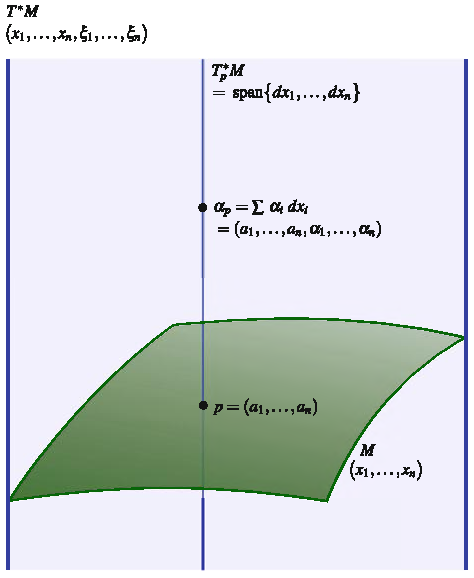
\includegraphics[width=0.656\linewidth]{images/vector/fig-B-5.pdf}
  \caption{余切丛 $T^*M$. 流形 $M$ 的坐标函数为 $(x_1,\ldots,x_n)$, 流形 $T^*M$ 的坐标函数为 $(x_1,\ldots,x_n,\xi_1,\ldots,\xi_n)$. 点 $p\in M$ 记为 $(a_1,\ldots,a_n)$, 点 $\alpha_p\in T^*M$ 记为 $(a_1,\ldots,a_n,\alpha_1,\ldots,\alpha_n)$. 注意, 由于 $M$ 的坐标函数是 $(x_1,\ldots,x_n)$, 余切空间 $T_p^*M$ 由 $\operatorname{span}\{dx_1,\ldots,dx_n\}$ 给出}
  \label{fig:B-5}
\end{figure}

我们要做的是把整个余切丛 $T^*M$ 看作我们的流形. 如果我们愿意, 可以把 $M=T^*M$ 写清楚. 虽然我们实际上不会这样做, 但记住现在我们是把整个余切丛当作流形、而不仅仅是底空间 $M$ 是很重要的. 这个新流形 $T^*M$ 的坐标函数是什么？记住, 本质上坐标给流形上的每个点一个"地址". 还要记住, 我们倾向于把坐标与坐标函数互换使用, 导致出现像
\[
x_1(p)=x_1,\quad x_2(p)=x_2,\quad\ldots,\quad x_n(p)=x_n
\]
这样的方程, 其中左边的 $x_i$ 是坐标函数, 右边的 $x_i$ 是用特定坐标片映射给点 $p$ 的数值"地址".

为了弄清楚流形 $T^*M$ 上的坐标是什么, 我们需要先问自己 $T^*M$ 中的点到底是什么. 但 $T^*M$ 中的点与 $T^*M$ 的元素是同一回事, 而我们知道那些是什么, $M$ 上某点 $p$ 处的微分 1-形式. 考虑 1-形式 $\alpha_p=\sum\alpha_i(dx_i)_p\in T_p^*M$, 其中 $x_1(p)=a_1,\ldots,x_n(p)=a_n$, 且 $\alpha_i$ 或是数或是 $M$ 上的函数. （在下面的讨论中我们将假设它们是数. 如果它们是函数, 那么在任意给定点, 只需在该点求值就能找到数值, 即 $\alpha_i(p)=\alpha_i$.）把 $p$ 写为 $p=(a_1,\ldots,a_n)$, 我们把 $T_p^*M$ 的基元素写为 $(dx_i)_p=(dx_i)_{(a_1,\ldots,a_n)}$. 把这些放在一起, 我们可以写
\[
\alpha_{(a_1,\ldots,a_n)}=\sum_{i=1}^{n}\alpha_i(dx_i)_{(a_1,\ldots,a_n)}.
\]
这个 1-形式完全由值 $a_1,\ldots,a_n$ 与值 $\alpha_1,\ldots,\alpha_n$ 决定. 于是我们可以把点 $\alpha_p$ 的"地址"定义为 $(a_1,\ldots,a_n,\alpha_1,\ldots,\alpha_n)$. 显然, 这个地址前半部分的坐标函数与 $M$ 上的坐标函数相同, 即 $x_1,\ldots,x_n$. 换言之, 
\[
x_1(\alpha_p)=a_1,\quad x_2(\alpha_p)=a_2,\quad\ldots,\quad x_n(\alpha_p)=a_n.
\]
后半部分呢？给出值 $\alpha_i$ 作为输出的坐标函数是什么？有时你会看到这些坐标函数记为 $dx_i$. 于是有
\[
dx_1(\alpha_p)=\alpha_1,\quad dx_2(\alpha_p)=\alpha_2,\quad\ldots,\quad dx_n(\alpha_p)=\alpha_n.
\]
当然, 现在 $dx_i$ 肯定不是在做我们一直期待 $dx_i$ 做的事, 即吃掉向量吐出数. 相反, $dx_i$ 们是在吃掉某点处的 1-形式, 吐出该 1-形式中对应于 $dx_i$ 的系数. 所以这里的 $dx_i$ 是坐标函数, 而不是微分 1-形式. 用这种记号, 我们说 $T^*M$ 上的坐标函数, 或坐标, 是 $(x_1,\ldots,x_n,dx_1,\ldots,dx_n)$.

作为例子, 考虑流形 $M=\mathbb{R}^3$ 与点 $(3,2,-1)\in\mathbb{R}^3$ 处的 1-形式
\[
\alpha_{(3,2,-1)}=5dx_1-4dx_2+6dx_3.
\]
那么 $T^*\mathbb{R}^3$ 的坐标函数, 或坐标, 是 $(x_1,x_2,x_3,dx_1,dx_2,dx_3)$, 如果你愿意, 也可以写成 $(x,y,z,dx,dy,dz)$. 于是有
\begin{align*}
x_1\left(\alpha_{(3,2,-1)}\right)=3,\qquad
x_2\left(\alpha_{(3,2,-1)}\right)=2,\qquad
x_3\left(\alpha_{(3,2,-1)}\right)=-1, \\
dx_1\left(\alpha_{(3,2,-1)}\right)=5,\qquad
dx_2\left(\alpha_{(3,2,-1)}\right)=-4,\qquad
dx_3\left(\alpha_{(3,2,-1)}\right)=6.
\end{align*}
因此 $\alpha_{(3,2,-1)}$ 可以"用坐标"写为 $(3,2,-1,5,-4,6)$.

鉴于我们花了很大力气强调微分 1-形式是吃掉向量吐出数的东西, 现在把它们想成流形 $T^*M$ 上吃掉流形的点（而这些点恰好本身是 1-形式）吐出实数系数的坐标函数, 似乎非常奇怪. 我们怎么分辨我们什么时候是把 $dx_i$ 想成 1-形式、什么时候想把它当成流形 $T^*M$ 上的坐标函数？人们可以说"从上下文辨别", 这常常就是实际情况, 但那似乎有点不公平. 相反, 我们要做的是把坐标函数版本的 $dx_i$ 重新命名为 $\xi_i$. 也就是说, 只有当我们把 $dx_1,\ldots,dx_n$ 想成 $T^*M$ 上的坐标函数时, 我们才使用 $\xi_1=dx_1,\ldots,\xi_n=dx_n$. 所以对我们的例子, 我们会有
\begin{align*}
x_1\left(\alpha_{(3,2,-1)}\right)=3,\qquad
x_2\left(\alpha_{(3,2,-1)}\right)=2,\qquad
x_3\left(\alpha_{(3,2,-1)}\right)=-1, \\
\xi_1\left(\alpha_{(3,2,-1)}\right)=5,\qquad
\xi_2\left(\alpha_{(3,2,-1)}\right)=-4,\qquad
\xi_3\left(\alpha_{(3,2,-1)}\right)=6.
\end{align*}
我们试着在图~\ref{fig:B-5} 中总结所有这些.

\begin{figure}[htbp]
  \centering
  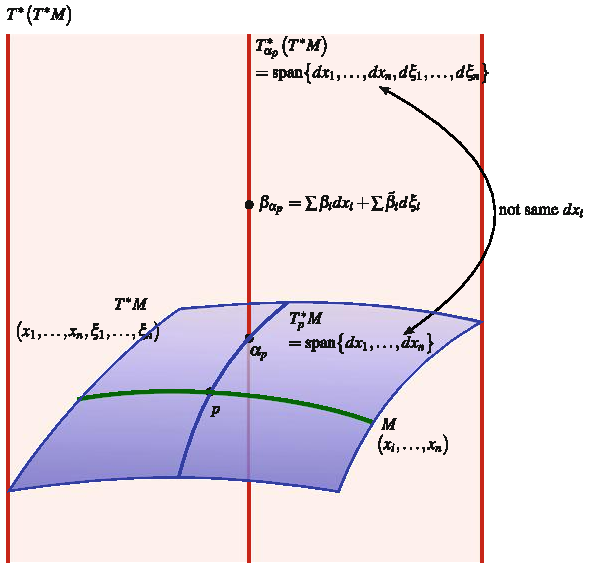
\includegraphics[width=0.816\linewidth]{images/vector/fig-B-6.pdf}
  \caption{余切丛 $T^*T^*M$. 流形 $M$ 的坐标函数为 $(x_1,\ldots,x_n)$, 流形 $T^*M$ 的坐标函数为 $(x_1,\ldots,x_n,\xi_1,\ldots,\xi_n)$. 流形 $T^*T^*M$ 的坐标函数未给出. $T_p^*M=\operatorname{span}\{dx_1,\ldots,dx_n\}$, 而 $T_{\alpha_p}^*T^*M=\operatorname{span}\{dx_1,\ldots,dx_n,d\xi_1,\ldots,d\xi_n\}$, 但请注意, 这两个空间的 $dx_i$ 并不相同}
  \label{fig:B-6}
\end{figure}

现在, 正如我们在流形 $M$ 上定义 1-形式一样, 我们可以在流形 $T^*M$ 上定义 1-形式. 流形 $T^*M$ 上的 1-形式实际上是 $T^*M$ 的余切丛的元素, 我们把它记为 $T^*T^*M$. 在图~\ref{fig:B-6} 中尝试画出了 $T^*M$ 的余切丛. 由于 $T^*M$ 上的坐标函数现在写成 $(x_1,\ldots,x_n,\xi_1,\ldots,\xi_n)$, 流形 $T^*M$ 的 1-形式基元素是 $dx_1,\ldots,dx_n,d\xi_1,\ldots,d\xi_n$. 这些是空间 $T^*(T^*M)$ 的基元素. 在特定点 $\alpha_p\in T^*M$ 处有
\[
(dx_1)_{\alpha_p},\ldots,(dx_n)_{\alpha_p},(d\xi_1)_{\alpha_p},\ldots,(d\xi_n)_{\alpha_p}\in T_{\alpha_p}^*(T^*M).
\]
注意, 作为流形 $T^*M$ 上 1-形式的 $dx_i$ 看起来就像作为流形 $M$ 上 1-形式的 $dx_i$.

我们将直接说明, 你需要学会从上下文辨认 $dx_i$ 什么时候是流形 $T^*M$ 上的 1-形式、什么时候是流形 $M$ 上的 1-形式. 否则我们的记号会变得极其复杂. 这也是当我们想认为 $dx_i$ 是流形 $T^*M$ 上的坐标函数时切换记号到 $\xi_i$ 的另一个原因. 让相同的记号 $dx_i$ 可能意味着三种不同的东西, 实在太多了.

既然我们已经开始掌握余切丛本身就是一个流形的想法, 并引入了余切丛的余切丛的想法, 让我们考虑 $T^*M$ 上的 1-形式, 即 $T^*T^*M$ 的元素, 会是什么样子. 它会有一般形式
\[
\beta=\sum_{i=1}^{n}\beta_idx_i+\sum_{i=1}^{n}\tilde{\beta}_id\xi_i,
\]
其中对 $i=1,\ldots,n$, $\beta_i$ 与 $\tilde{\beta}_i$ 或是数或是 $T^*M$ 上的函数, $\beta_i:T^*M\to\mathbb{R}$ 且 $\tilde{\beta}_i:T^*M\to\mathbb{R}$. 但这正是我们的坐标函数 $x_i$ 与 $\xi_i$ 所是的, $T^*M$ 上的函数. 即 $x_i:T^*M\to\mathbb{R}$ 且 $\xi_i:T^*M\to\mathbb{R}$. 如果我们令 $\beta_i=\xi_i$、$\tilde{\beta}_i=0$, 那么我们就得到 $T^*M$ 上一个非常特殊的 1-形式, 称为\newterm{liouville-one-form}{Liouville 1-形式}{Liouville one-form}, 我们把它记为 $\alpha$：
\[
\text{Liouville 1-形式：}\qquad\alpha=\sum_{i=1}^{n}\xi_idx_i.
\]
在头脑中把一切都理顺很重要：$\xi_i:T^*M\to\mathbb{R}$ 是流形 $T^*M$ 上的坐标函数, 而 $dx_i$ 是流形 $T^*M$ 上的 1-形式, 这意味着 $dx_i\in T^*T^*M$. Liouville 1-形式也称为恒等 1-形式或典范 1-形式. 这个 1-形式总是存在于流形 $T^*M$ 上.

Liouville 1-形式可以用来在流形 $T^*M$ 上得到一个 2-形式. 我们通过取 Liouville 1-形式的外微分做到这一点, 
\[
d\alpha=\sum_{i=1}^{n}d\xi_i\wedge dx_i=-\sum_{i=1}^{n}dx_i\wedge d\xi_i.
\]
注意现在 $dx_i$ 与 $d\xi_i$ 都是流形 $T^*M$ 上的 1-形式, 即 $dx_i,d\xi_i\in T^*T^*M$. 注意这正是流形 $T^*M$ 上的一个辛形式. 我们把 $T^*M$ 上的\newterm{canonical-symplectic-form}{典范辛形式}{canonical symplectic form}定义为
\[
\text{典范辛形式：}\qquad\omega\equiv-d\alpha=\sum_{i=1}^{n}dx_i\wedge d\xi_i,
\]
其中 $\alpha$ 是 $T^*M$ 上的 Liouville 1-形式. 这里出现负号的唯一真正原因是让我们的 2-形式元素的顺序与我们喜欢写坐标的顺序一致.

还有另一种引入典范辛形式的常用方式. 假设我们有把余切丛投影到其底流形的投影映射 $\pi$：
\[
\begin{array}{c}T^*M\\\big\downarrow\pi\\M\end{array}
\]
这个映射取 $T^*M$ 中的任何元素 $\xi_p\in T^*M$（它是 $M$ 上某点 $p$ 处的 1-形式）, 并把它投影到基点 $\pi(\xi_p)=p$. 正如我们已经讨论过的, 正如流形 $M$ 有切空间 $TM$ 一样, 流形 $T^*M$ 也有切空间 $T(T^*M)$. 假设 $v_{\xi_p}$ 是以 $\xi_p\in T^*M$ 为基点的流形 $T^*M$ 上的向量. 与所有流形之间的映射一样, 投影映射 $\pi:T^*M\to M$ 诱导切丛之间的前推映射
\[
T(T^*M)\xrightarrow{\pi_*}TM,
\]
它把向量 $v_{\xi_p}\in T_{\xi_p}(T^*M)$ 前推到点 $p$ 处 $TM$ 中的向量, 即 $\pi_*(v_{\xi_p})\in T_pM$.

正如我们定义投影 $\pi:T^*M\to M$ 一样, 我们可以定义投影
\[
\begin{array}{c}T(T^*M)\\\big\downarrow\Pi\\T^*M\end{array}
\]
为 $\Pi(v_{\xi_p})=\xi_p$. 你应该知道, 通常所有投影映射都简单地记为 $\pi$, 你需要从上下文弄清楚哪个空间被投影到哪个流形. 但这里我们区分所用的两个投影：$\pi:T^*M\to M$ 与 $\Pi:T(T^*M)\to T^*M$.

类似地, 流形 $T^*M$ 也有余切丛 $T^*T^*M$, 其元素是 $T^*M$ 上吃掉向量 $v_{\xi_p}\in T(T^*M)$ 的 1-形式. 我们按如下方式在 $T^*T^*M$ 中定义一个 1-形式 $\alpha$：
\[
\text{Liouville 1-形式：}\qquad\alpha(v_{\xi_p})\equiv\Pi(v_{\xi_p})\bigl(\pi_*(v_{\xi_p})\bigr)=\bigl\langle\Pi(v_{\xi_p}),\pi_*(v_{\xi_p})\bigr\rangle,
\]
其中 $\langle\cdot,\cdot\rangle$ 只是写 1-形式与向量之间\newterm{canonical-pairing}{典范配对}{canonical pairing}的另一种方式. 这个 $\alpha$ 正是 Liouville 1-形式. 我们在图~\ref{fig:B-7} 中说明 Liouville 1-形式的这个定义. 典范辛形式就是 Liouville 1-形式的外微分的负值, $\omega=-d\alpha$.

\begin{figure}[htbp]
  \centering
  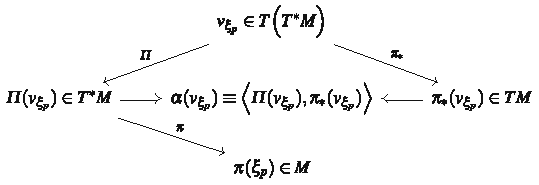
\includegraphics[width=0.745\linewidth]{images/vector/fig-B-7.pdf}
  \caption{Liouville 1-形式 $\alpha$ 用向量 $v_{\xi_p}$ 内蕴地定义. 由 $\pi(\xi_p)=p$ 定义的投影映射 $\pi:T^*M\to M$ 诱导前推映射 $\pi_*:T(T^*M)\to TM$. 映射 $\Pi$ 也是投影映射, $\Pi:T(T^*M)\to T^*M$, 由 $\Pi(v_{\xi_p})=\xi_p$ 定义. 吃掉向量 $v_{\xi_p}$ 的 Liouville 1-形式 $\alpha$ 由 1-形式 $\Pi(v_{\xi_p})$ 与向量 $\pi_*(v_{\xi_p})$ 的典范配对定义. 注意在这个定义中任何地方都没有用到实际的流形坐标. 典范辛形式就是 Liouville 1-形式的外微分的负值, $\omega=-d\alpha$}
  \label{fig:B-7}
\end{figure}

但这是一个多么奇怪的定义——基本上似乎一切都在用单个向量, 即向量 $v_{\xi_p}\in T(T^*M)$ 来定义. 但注意一些有趣的事情：在这个定义的任何地方, 我们都没有用到任何流形的实际坐标. 我们能够内蕴地定义 Liouville 1-形式, 即不参照流形坐标. 我们以前提到过这一点. 数学家喜欢内蕴的、坐标无关的定义, 因为这些定义常常使底层的数学结构更容易看清, 也常常使证明事情更容易. 然而, 当落实到实际计算时, 人们通常需要涉及坐标的公式.

假设我们在 $M$ 上有坐标 $(x_1,\ldots,x_n)$, 并且我们有 1-形式 $\xi_p=\sum_{i=1}^{n}\xi_idx_i\in T^*M$, 它给出 $T^*M$ 上的坐标 $(x_1,\ldots,x_n,\xi_1,\ldots,\xi_n)$. 我们常把这些坐标分别简写为 $(x_i)$ 与 $(x_i,\xi_i)$. 用这些坐标, 投影映射是 $\pi(x_1,\ldots,x_n,\xi_1,\ldots,\xi_n)=(x_1,\ldots,x_n)$, 或 $\pi(x_i,\xi_i)=x_i$.

\section{Darboux 定理}

这是一本关于微分形式、而不是流形理论的书, 所以我们一直在考虑的只是"好的"流形, 即可微流形. 可微流形 $M$ 是局部上足够类似于 $\mathbb{R}^n$、从而可以在其上做微积分的流形. 这意味着流形有一个带坐标图 $(U_i,\varphi_i)$ 的图册, 其中 $\varphi_i:U_i\subset\mathbb{R}^n\to M$ 光滑, $\varphi_i^{-1}$ 存在, 且所有 $\varphi_i^{-1}\circ\varphi_j$ 都是可微映射.

辛流形是可微流形的特殊情形. 我们已经说过, 辛流形 $M$ 在其上处处定义了辛形式, 其中辛形式是闭非退化 2-形式. 我们还看了一个辛形式的例子, $\sum_{i=1}^{n}dx_i\wedge dy_i$, 其中 $(x_1,\ldots,x_n,y_1,\ldots,y_n)$ 是坐标函数. 由于这个形式显然定义在 $\mathbb{R}^{2n}$ 上处处成立, 我们可以看到 $\mathbb{R}^{2n}$ 总是辛流形.

Darboux 定理断言：在辛流形 $(M,\omega)$ 上任何一点的邻域内, 都可以选择坐标 $(x_1,\ldots,x_n,y_1,\ldots,y_n)$, 使得我们可以把 $\omega$ 写成
\[
\omega=\sum_{i=1}^{n}dx_i\wedge dy_i.
\]
本质上, Darboux 定理所暗示的是所有辛形式 $\omega$ 本质上相同. 这很好, 因为它意味着总有可能选择坐标, 使得我们可以把辛形式写成 $\sum_{i=1}^{n}dx_i\wedge dy_i$. 为了证明 Darboux 定理, 我们将使用通常称为 Moser 技巧或 Moser 引理的东西. Moser 引理有若干版本, 但我们将坚持对我们这里的目的而言最简单的版本.

\begin{lemma}[Moser 引理]\label{lem:B-1}
设 $\{\omega_t\}$（$0\leq t\leq1$）是流形 $M$ 上的一族辛形式. 那么对每个点 $p\in M$, 存在 $p$ 的邻域 $U$ 和函数 $g_t:U\to U$, 使得 $g_0^*$ 是恒等函数, 并且对所有 $0\leq t\leq1$ 有 $g_t^*\omega_t=\omega_0$.
\end{lemma}

我们的目标当然是求映射 $g_t:U\to U$. 但考虑图~\ref{fig:A-1}, 它显示了向量场 $v$ 的积分曲线 $\gamma_t$. 另一种说法是
\[
\frac{d}{dt}\gamma_t(p)=v\left(\gamma_t(p)\right).
\]
所以如果我们知道向量场 $v$ 是什么, 我们就可以对 $v$ 积分得到积分曲线 $\gamma_t$, 后者是时间的函数. 此外, 在每个时刻 $t$, $\gamma_t$ 都是流形到自身的映射, 即 $\gamma_t:M\to M$. 这本质上就是 Moser 引理中使用的策略；找到一个向量场 $v$, 然后给出满足 $g_0^*=\mathrm{id}$ 与 $g_t^*\omega_t=\omega_0$ 的积分曲线 $g_t:U\to U$. 找到这个向量场恰好需要辛形式 $\omega_t$ 所具有的两个性质, 闭性与非退化性.

我们要证明的第一件事是稍后不久会需要的某个东西. 由于 $\omega_t$ 是辛形式, 我们知道它是闭的, $d\omega_t=0$. 我们想证明 $\frac{d}{dt}\omega_t$ 也是闭的. 我们不知道 $\omega_t$ 取什么形式, 但至少我们知道它是 2-形式, 所以我们可以用坐标把它写成
\[
\omega_t=\sum_{i<j}f_{i,j}(t)\,dx_i\wedge dx_j.
\]
于是有
\[
\begin{aligned}
d\left(\frac{d}{dt}\omega_t\right)&=d\left(\frac{d}{dt}\sum_{i<j}f_{i,j}(t)\,dx_i\wedge dx_j\right)\\
&=\sum_{i<j}\frac{d}{dt}f_{i,j}(t)\,d\left(dx_i\wedge dx_j\right)\\
&=\frac{d}{dt}\sum_{i<j}f_{i,j}(t)\,d\left(dx_i\wedge dx_j\right)\\
&=\frac{d}{dt}d\left(\sum_{i<j}f_{i,j}(t)\,dx_i\wedge dx_j\right)\\
&=\frac{d}{dt}d\omega_t\\
&=0.
\end{aligned}
\]
利用 Poincaré 引理, 我们知道 $\frac{d}{dt}\omega_t$ 是恰当的, 所以存在 1-形式 $\lambda_t$ 使得
\[
\frac{d}{dt}\omega_t=d\lambda_t.
\]
我们做的下一件事是对 $g_t^*\omega_t$ 关于时间求导. 这给出
\[
\begin{aligned}
\frac{d}{dt}g_t^*\omega_t&=\lim_{h\to0}\frac{g_{t+h}^*\omega_{t+h}-g_t^*\omega_t}{h}\\
&=\lim_{h\to0}\frac{g_{t+h}^*\omega_{t+h}-g_t^*\omega_{t+h}+g_t^*\omega_{t+h}-g_t^*\omega_t}{h}\\
&=\lim_{h\to0}\frac{g_{t+h}^*\omega_{t+h}-g_t^*\omega_{t+h}}{h}+\lim_{h\to0}\frac{g_t^*\omega_{t+h}-g_t^*\omega_t}{h}\\
&=g_t^*\lim_{h\to0}\frac{g_h^*\omega_{t+h}-\omega_{t+h}}{h}+g_t^*\lim_{h\to0}\frac{\omega_{t+h}-\omega_t}{h}\\
&=g_t^*L_{v_t}\omega_t+g_t^*\frac{d\omega_t}{dt}\\
&=g_t^*L_{v_t}\omega_t+\frac{d\omega_t}{dt}\\
&=g_t^*\left(d\iota_{v_t}\omega_t+d\lambda_t\right)\\
&=g_t^*d\left(\iota_{v_t}\omega_t+\lambda_t\right).
\end{aligned}
\]
在上面这个计算中有几个小的细节应该说明一下. 首先, 
\[
L_{v_t}\omega_t=\lim_{h\to0}\frac{g_h^*\omega_{t+h}-\omega_{t+h}}{h}
\]
可能看起来与第 A.7 节给出的 Lie 导数定义有点不同, 但这里我们没有跟踪基点. 第二, 我们使用了 Cartan 同伦公式以及 $\omega_t$ 是闭的这一事实得到
\[
L_{v_t}\omega_t=\iota_{v_t}(d\omega_t)+d(\iota_{v_t}\omega_t)=d\iota_{v_t}\omega_t.
\]

我们想让我们的函数 $g_t$ 满足等式 $g_t^*\omega_t=\omega_0$. 关于时间求导, 我们发现这等价于
\[
\frac{d}{dt}g_t^*\omega_t=\frac{d}{dt}\omega_0=0.
\]
代入我们刚找到的恒等式, 这又等价于
\[
g_t^*d\left(\iota_{v_t}\omega_t+\lambda_t\right)=0,
\]
而如果
\[
\iota_{v_t}\omega_t+\lambda_t=0,
\]
则这是真的. 这有时称为 Moser 方程. 如果我们能对 $v$ 解出这个方程, 那么我们就能求 $v$ 的积分曲线, 得到满足所要求的 $g_t^*\omega_t=\omega_0$ 的映射 $g_t$. 注意, 如果这个成立, 那么 $g_0$ 平凡地是恒等函数.

所以现在我们的目标变成解方程 $\iota_v\omega_t+\lambda_t=0$. 假设 $M$ 是以 $(x_1,\ldots,x_{2n})$ 为局部坐标的 $2n$ 维流形. 令 $\frac{\partial}{\partial x_k}$ 为 $TM$ 的基、$dx_k$ 为 $T^*M$ 的基, 我们可以写
\begin{align*}
\lambda_t=\sum_{i=1}^{2n}\lambda_i(t,x)\,dx_i, \\
v_t=\sum_{k=1}^{2n}v_k(t,x)\frac{\partial}{\partial x_k}, \\
\omega_t=\sum_{\substack{k,\ell=1\\k<\ell}}^{2n}\omega_{k,\ell}(t,x)\,dx_k\wedge dx_\ell.
\end{align*}
利用这个我们可以写
\[
\iota_{v_t}\omega_t=2\sum_{\ell=1}^{2n}\left(\sum_{k=1}^{2n}\omega_{k,\ell}(t,x)v_k(t,x)\right)dx_\ell,
\]
并把 $\iota_{v_t}\omega_t+\lambda_t=0$ 写为
\[
2\sum_{\ell=1}^{2n}\left(\sum_{k=1}^{2n}\omega_{k,\ell}(t,x)v_k(t,x)\right)dx_\ell+\sum_{\ell=1}^{2n}\lambda_\ell(t,x)\,dx_\ell=0.
\]
这实际上给出一个由 $2n$ 个方程组成的方程组
\[
\lambda_\ell(t,x)+2\sum_{k=1}^{2n}\omega_{k,\ell}(t,x)v_k(t,x)=0,
\]
当然可以写成
\begin{align*}
\lambda_1(t,x)+2\sum_{k=1}^{2n}\omega_{k,1}(t,x)v_k(t,x)=0, \\
\lambda_2(t,x)+2\sum_{k=1}^{2n}\omega_{k,2}(t,x)v_k(t,x)=0, \\
\vdots \\
\lambda_{2n}(t,x)+2\sum_{k=1}^{2n}\omega_{k,2n}(t,x)v_k(t,x)=0,
\end{align*}
这又可以写成矩阵形式
\[
\begin{bmatrix}\lambda_1\\\vdots\\\lambda_{2n}\end{bmatrix}
+2\underbrace{\begin{bmatrix}\omega_{1,1}&\cdots&\omega_{2n,1}\\\vdots&\ddots&\vdots\\\omega_{1,2n}&\cdots&\omega_{2n,2n}\end{bmatrix}}_{\Omega}
\begin{bmatrix}v_1\\\vdots\\v_{2n}\end{bmatrix}=0,
\]
或更简洁地写成
\[
\lambda+2\Omega v=0.
\]
由于对 $0\leq t\leq1$, $\omega_t$ 是辛形式, 它是非退化的, 这意味着矩阵 $\Omega$ 是非奇异的, 从而可以求逆. 如果你没有上过线性代数课, 这可能让你不清楚, 但我们不会在这里尝试解释这个细节, 而是把你引向一本线性代数教科书. 但这个事实允许我们解出 $v$：
\[
v=-\frac{1}{2}\Omega^{-1}\lambda.
\]
于是我们找到唯一的向量场 $v_t$ 作为 Moser 方程 $\iota_{v_t}\omega_t+\lambda_t=0$ 的解. 然后这个向量场 $v_t$ 可以被积分, 给出积分曲线 $g_t$, 它们正是我们需要找的映射, 从而证明了 Moser 引理. 手头有了 Moser 引理, Darboux 定理的证明就几乎平凡了.

\begin{theorem}[Darboux 定理]\label{thm:B-1}
如果 $(M,\omega)$ 是 $2n$ 维辛流形, 那么在每个点 $p\in M$ 的邻域 $U$ 中存在局部坐标 $(x_1,\ldots,x_n,y_1,\ldots,y_n)$, 使得辛形式 $\omega$ 可以写成
\[
\omega=\sum_{i=1}^{n}dx_i\wedge dy_i.
\]
\end{theorem}

给定辛形式 $\omega$, 那么在 $M$ 上的任何点 $p$ 处都可以找到局部坐标
\[
(x_1',\ldots,x_n',y_1',\ldots,y_n'),
\]
使得
\[
\omega\bigl|_p=\sum_{i=1}^{n}dx_i'\wedge dy_i'\Bigr|_p.
\]
这相当直接地可以看出. 任何坐标片上都会有一个 $\sum_{i=1}^{n}dx_i'\wedge dy_i'$ 形式的辛形式. 只需缩放坐标, 直到在点 $p$ 处得到等式. 当然在此时, 没有理由期待 $\omega$ 会在 $U$ 上（而非 $p$ 处）等于 $\sum_{i=1}^{n}dx_i'\wedge dy_i'$.

所以现在我们在 $U$ 上有两个辛形式, $\omega_0=\omega$ 与 $\omega_1=\sum_{i=1}^{n}dx_i'\wedge dy_i'$. 我们可以用它们来定义形式族 $\{\omega_t\}$：
\[
\omega_t=\omega_0+t(\omega_1-\omega_0).
\]
当然, 由于 $\omega_0$ 与 $\omega_1$ 都是辛形式, 自然会假设对每个 $t$ 的 $\omega_t$ 也是. 但这是必须检验的东西. 由于 $\omega_0$ 与 $\omega_1$ 都是辛形式, 它们是闭的, 所以容易看出 $\omega_t$ 也是闭的：
\[
d\omega_t=\underbrace{d\omega_0}_{=0}+t\left(\underbrace{d\omega_1}_{=0}-\underbrace{d\omega_0}_{=0}\right)=0.
\]
证明 $\omega_t$ 非退化需要多一点功夫, 这就是我们不辞辛劳地找到满足 $\omega_1(p)=\omega_0(p)$ 的 $\omega_1$ 的原因. 这意味着 $\omega_t(p)$ 实际上与 $t$ 无关. 换言之, 对 $0\leq t\leq1$ 有 $\omega_t(p)=\omega_0(p)=\omega_1(p)$. 由于我们定义 $\omega_t=\omega_0+t(\omega_1-\omega_0)$, 我们看到 $\omega_t$ 是 $\omega_0$ 与 $\omega_1$ 的连续函数. 换言之, 随着 $t$ 从 0 到 1, $\omega_t$ 从 $\omega_0$ 连续变化到 $\omega_1$. 由于 $\omega_0$ 与 $\omega_1$ 在 $p$ 的邻域中都是非退化的, 那么由 $\omega_t$ 的连续性, 对 0 到 1 之间的所有 $t$, $\omega_t$ 在 $p$ 的某个邻域中都是非退化的, 因此对 $0\leq t\leq1$ 是辛形式. "由连续性"这个说法对你来说可能看起来奇怪. 这基本上指的是连续函数所具有的性质, 这通常是在分析或泛函分析课程中学习的. 同样, 我们不会在这里尝试更详细地解释这一点, 而是把你引向一本分析教科书.

所以对每个 $t\in[0,1]$, $\omega_t$ 既是闭的又是非退化的, 因此 $\{\omega_t\}$ 是一族辛形式, 所以我们可以应用 Moser 引理. 根据 Moser 引理, 在点 $p\in M$ 周围的某个邻域 $U$ 中存在映射 $g_t:U\to U$, 使得 $g_t^*\omega_t=\omega_0$. 特别地, 我们有 $g_1^*\omega_1=\omega_0$. 换言之, 
\[
\omega=g_1^*\left(\sum_{i=1}^{n}dx_i'\wedge dy_i'\right)=\sum_{i=1}^{n}d(x_i'\circ g_1)\wedge d(y_i'\circ g_1).
\]
我们现在选择新坐标 $x_i=x_i'\circ g_1$ 与 $y_i=y_i'\circ g_1$, 从而证明了 Darboux 定理.

\section{几何力学浅尝}

在本节中我们给出几何力学的非常简短的介绍. 我们将说明, 可以把简单力学系统的 Hamiltonian 方程写成用辛形式表示的形式. 我们不会讲太多细节, 所以我们将只陈述、而不展示一个非常重要的对应关系. 本节的目的在于看看余切丛上的典范辛 2-形式在哪里以及如何被使用. 你可能跟不上每一个细节, 但那没关系, 现在仅仅把握大局就足够了.

在物理和力学中, 我们实际使用的流形来自我们所考虑的具体物理问题. 例如, 如果我们考虑一个在地球引力作用下的点粒子的非常简单的物理系统, 我们所关心的流形来自粒子的 $x$、$y$ 与 $z$-坐标. 所以我们的流形是坐标为 $(x,y,z)$ 的 $M=\mathbb{R}^3$. 如果我们考虑一个由 $n$ 个粒子组成的、远离地球、彼此之间都受引力影响的系统, 那么我们所关心的是这些粒子中每一个的 $x$、$y$ 与 $z$-坐标, 所以我们的流形是坐标为 $(x_1,y_1,z_1,x_2,y_2,z_2,\ldots,x_n,y_n,z_n)$ 的 $M=\mathbb{R}^{3n}$.

在物理和力学中, 来自物理系统的流形称为该物理系统的\newterm{configuration-space}{位形空间}{configuration space}. 当然, 正如你很可能从物理课上知道的, 如果选择正确的坐标系, 你可以相当大地简化你的流形. 这里我们不会担心这一点, 只说当我们能够基于所考虑的实际物理系统的对称性或其他性质对流形做出简化时, 该流形仍被称为位形空间, 但我们的坐标通常被称为\newterm{generalized-coordinates}{广义坐标}{generalized coordinates}. 当我们考虑广义坐标, 或者就这一点而言, 位形空间的任何坐标时, 记号约定是使用变量 $q$ 而不是变量 $x$. 于是我们说流形有坐标（或坐标函数）$(q_1,q_2,\ldots,q_n)$. 如果你看到 $q$ 被用作流形的坐标函数而不是 $x$, 你可以相当确信这本书或这篇论文是从物理或力学的视角写的, 而且所用的技巧很可能对物理或力学系统有用.

现在我们转向\newterm{flow}{流}{flow}的思想. 流本质上与积分曲线是同一个东西, 例如参见图~\ref{fig:2-4}, 只不过出现在物理或力学问题的语境中. 假设你有一个流形 $M$, 并且它上面有一个"流". 你可以把流形中的流想象成正在流过流形的流体. 流体的每个粒子确定 $M$ 上的一条轨迹. 流形上的流被描绘为 $M$ 上流体粒子轨迹的集合, 见图~\ref{fig:B-8}.

\begin{figure}[htbp]
  \centering
  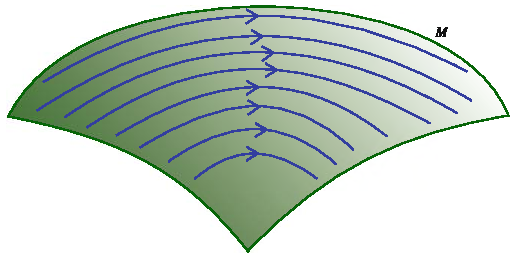
\includegraphics[width=0.714\linewidth]{images/vector/fig-B-8.pdf}
  \caption{画有几条流轨道的流形 $M$}
  \label{fig:B-8}
\end{figure}

当流体流动时, 在每个时刻流体的每个粒子都有一个速度, 从而有一个速度向量. 例如, 在时刻 $t_0$, $M$ 中所有点的所有粒子都有一个速度. 在时刻 $t_0$ 的这一组速度向量给出 $M$ 上的速度向量场 $v_{t_0}$；即 $v_{t_0}$ 是 $TM$ 中的截面. 类似地, 在更晚的时刻 $t_1$, 在 $M$ 中流动的粒子产生速度向量场 $v_{t_1}$, 它当然也是 $TM$ 中的截面. 见图~\ref{fig:B-9}.

\begin{figure}[htbp]
  \centering
  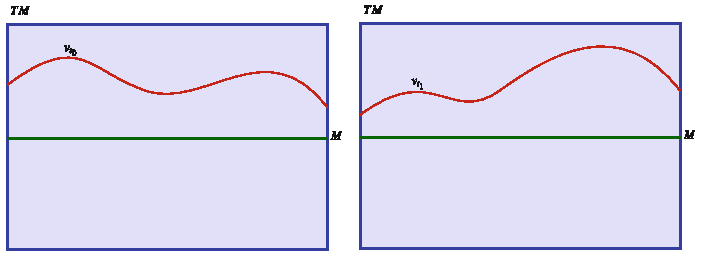
\includegraphics[width=0.960\linewidth]{images/vector/fig-B-9.pdf}
  \caption{带截面 $v_{t_0}$（左）与截面 $v_{t_1}$（右）的切丛 $TM$}
  \label{fig:B-9}
\end{figure}

让我们在 $M$ 上单独挑出一条流线并仔细看看它, 如图~\ref{fig:B-10} 上图所示. 流的轨迹给出 $M$ 上的一条曲线. 我们把这条曲线记为
\[
q(t)=\left(q_1(t),q_2(t),\ldots,q_n(t)\right).
\]
在时刻 $t_0$, 曲线的速度向量由
\[
\dot{q}(t_0)=\left(\dot{q}_1(t_0),\dot{q}_2(t_0),\ldots,\dot{q}_n(t_0)\right)
=\left(\left.\frac{\partial q_1(t)}{\partial t}\right|_{t_0},\left.\frac{\partial q_2(t)}{\partial t}\right|_{t_0},\ldots,\left.\frac{\partial q_n(t)}{\partial t}\right|_{t_0}\right)
\]
给出. 这个速度向量 $\dot{q}(t_0)$ 位于点 $q(t_0)$ 处. 我们用完全相同的方式得到更晚时刻 $t_1$ 的速度向量. 见图~\ref{fig:B-10}.

\begin{figure}[htbp]
  \centering
  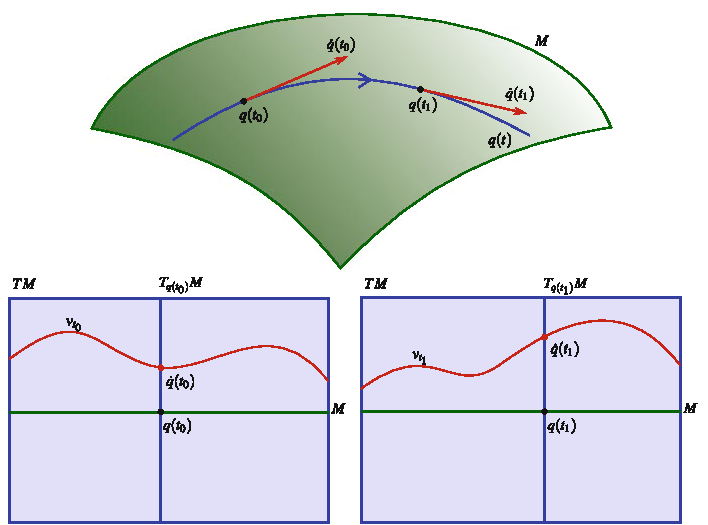
\includegraphics[width=0.960\linewidth]{images/vector/fig-B-10.pdf}
  \caption{上图：带单条流轨道 $q(t)=\left(q_1(t),q_2(t),\ldots,q_n(t)\right)$ 的流形 $M$. 在点 $q(t_0)$ 处显示了速度向量 $\dot{q}(t_0)$, 在点 $q(t_1)$ 处显示了速度向量 $\dot{q}(t_1)$. 下图：点 $q(t_0)$ 与 $q(t_1)$ 连同向量 $\dot{q}(t_0)$ 与 $\dot{q}(t_1)$ 显示在向量丛 $TM$ 中}
  \label{fig:B-10}
\end{figure}

所以, 如果我们以某种方式知道了某个流 $q$ 的速度向量场 $\dot{q}(t)$, 并且我们想求这个流 $q$ 的实际曲线, 我们就需要对 $\dot{q}$ 积分；即
\[
q(t)=\int\dot{q}(t)\,dt.
\]
于是流曲线 $q$ 是速度向量场 $\dot{q}$ 的积分曲线. 我们甚至不会假装在这里对一个真实例子做这件事, 但一般的抽象想法应当相对清楚——一个流的速度向量场可以被积分得到这个流. 所以, 如果我们有某种好的方式知道一个流的速度向量场, 那么得到实际的流就相对直接了.

现在我们考虑 $\mathbb{R}^3$ 中单个粒子的简单例子, 为简单起见, 我们假设无论使用什么单位, 它的质量都是一. 这是数学家几乎总是会做的假设, 物理学家有时会做, 值得庆幸的是工程师从不做. 我们还将基本上假装这个粒子没有体积, 它只是一个质量为 1 的点. 这是另一个常做的简化假设, 当这样做时, 该粒子被称为\newterm{point-mass}{质点}{point mass}. 这个质点的坐标由 $q=(q_1,q_2,q_3)$ 给出. 同样, 作为简化记号的一部分, 坐标常常就写成 $q$, 但需要理解这个 $q$ 实际上意味着 $(q_1,q_2,q_3)$.

我们将假设这个质点受到某个力的作用, 我们把它记为 $F$. 常常作用在粒子上的力取决于粒子的位置, 因此写成坐标的函数 $F(q)$. 如果力也是时间的函数, 那么我们就写 $F(q,t)$. 常常力 $F$ 可以写成用所谓的\newterm{potential-function}{势函数}{potential function}来表示, 势函数通常记为 $U$. 这不是物理课, 这只是对几何力学的一个非常简短的介绍, 所以我们不会深入讨论势函数. 这一切对我们来说意味着, 我们可以把力 $F$ 用势函数 $U$ 写成
\[
F(q)=-\frac{\partial U(q)}{\partial q}\qquad\text{或}\qquad F(q,t)=-\frac{\partial U(q,t)}{\partial q}.
\]
我们常说力 $F$ 来自势函数 $U$.

我们将假设在我们的例子中情形正是如此, 即力 $F$ 来自势函数 $U$. 那么在 $\mathbb{R}^3$ 中单个质点这个例子中, 方程 $F(q,t)=-\frac{\partial U(q,t)}{\partial q}$ 实际上意味着什么？回忆实际上 $q=(q_1,q_2,q_3)$, 所以方程 $F(q,t)=-\frac{\partial U(q,t)}{\partial q}$ 实际上意味着方程组
\begin{align*}
F_1(q_1,q_2,q_3,t)=-\frac{\partial U(q_1,q_2,q_3,t)}{\partial q_1}, \\
F_2(q_1,q_2,q_3,t)=-\frac{\partial U(q_1,q_2,q_3,t)}{\partial q_2}, \\
F_3(q_1,q_2,q_3,t)=-\frac{\partial U(q_1,q_2,q_3,t)}{\partial q_3},
\end{align*}
其中 $F_i$ 是 $q_i$ 方向上的力的分量.

由牛顿定律我们知道 $F=ma$, 其中 $m$ 是质量, $a$ 是加速度. 当然, 我们假设 $m=1$, 所以用这个简化假设我们可以写 $F=a$. 但我们也知道加速度只是速度的导数, 所以对我们的粒子有
\[
a=\ddot{q}=\frac{\partial^2q(t)}{\partial t^2},
\]
结果
\[
F=a\quad\Rightarrow\quad\ddot{q}(t)=-\frac{\partial U(q,t)}{\partial q},
\]
这显然是一个二阶微分方程. 实际上, 和上面的力一样, 它实际上是三个二阶微分方程组成的方程组：
\begin{align*}
\ddot{q}_1(t)=-\frac{\partial U(q_1,q_2,q_3,t)}{\partial q_1}, \\
\ddot{q}_2(t)=-\frac{\partial U(q_1,q_2,q_3,t)}{\partial q_2}, \\
\ddot{q}_3(t)=-\frac{\partial U(q_1,q_2,q_3,t)}{\partial q_3},
\end{align*}
其中 $\ddot{q}_i$ 是 $q_i$ 方向上的加速度分量.

在物理中, \newterm{momentum}{动量}{momentum}被定义为 $p=m\dot{q}=\dot{q}$, 其中最后一个等号是因为 $m=1$. 在我们的记号中计入对时间的依赖, 我们会写 $p(t)=\dot{q}(t)$. 和势函数一样, 我们不会被引入歧途去描述或解释动量是什么或它为什么重要, 对我们来说, 我们将简单地用数学方式使用它, 把我们的二阶常微分方程变成一阶常微分方程组：
\begin{align*}
\dot{q}(t)=p(t), \\
\dot{p}(t)=-\frac{\partial U(q,t)}{\partial q}.
\end{align*}
同样, 和上面的 $F$ 与 $\ddot{q}$ 一样, 这实际上是一组六个一阶常微分方程.

系统的总能量是粒子的势能与动能之和. 位于 $q$、时刻 $t$ 的粒子的势能由势函数 $U(q,t)$ 给出, 而粒子的动能由 $\frac{1}{2}p(t)\equiv\frac{1}{2}p^2(t)$ 给出. 于是总能量（记为 $H_t$）由
\[
H_t(p,q,t)=\frac{1}{2}p^2(t)+U(q,t)
\]
给出. 总能量函数是所谓的\newterm{hamiltonian-function}{Hamiltonian 函数}{Hamiltonian function}的一个例子, 这就是为什么我们用 $H$ 记它, 而记号中包含下标 $t$ 是为了帮助我们记住该函数对时间的依赖. 我们可以对 $H_t$ 关于 $p$ 和 $q$ 求导. 这样做并与上面的方程组等式结合, 我们得到
\begin{align*}
\frac{\partial H_t}{\partial p}=\frac{\partial}{\partial p}\left(\frac{1}{2}p^2(t)+U(q,t)\right)=p=\dot{q}, \\
\frac{\partial H_t}{\partial q}=\frac{\partial}{\partial q}\left(\frac{1}{2}p^2(t)+U(q,t)\right)=\frac{\partial U(q,t)}{\partial q}=-\dot{p}.
\end{align*}
于是上面的一阶微分方程组可以用 Hamiltonian 函数写成
\begin{align*}
\dot{q}=\frac{\partial H_t}{\partial p}, \\
\dot{p}=-\frac{\partial H_t}{\partial q}.
\end{align*}
这个方程组被称为\newterm{hamiltonian-equations}{Hamiltonian 方程}{Hamiltonian equations}. 在每个特定的时刻 $t$, 这些方程给我们一个速度向量 $(\dot{q},\dot{p})$. Hamiltonian 方程描述我们的质点粒子在来自势函数 $U$ 的力 $F$ 作用下的运动. 换言之, 通过求解这个方程组, 我们可以得到粒子的运动. 事实证明, 几乎任何物理系统都有一个 Hamiltonian 函数, 可以用来写出该系统的 Hamiltonian 方程.

实际上, 我们现在不再只有变量 $q$, 而是有了变量 $q$ 与 $p$. 通过增加变量的个数, 我们把二阶微分方程变成了一阶微分方程组. 这使得求解微分方程更容易, 但代价是需要解更多变量. 所以我们现在不再只有位形坐标 $q$, 而是有了动量坐标 $p$. 位形坐标与动量坐标合在一起给出所谓的系统的\newterm{phase-space}{相空间}{phase space}流形. 在我们的例子中, 相空间流形是坐标为 $(q_1,q_2,q_3,p_1,p_2,p_3)$ 的 $\mathbb{R}^6$.

让我们暂时离题, 想想这个动量 $p$ 到底是什么. 回忆, 我们把它定义为 $p=m\dot{q}$. 还要回忆, 我们声称粒子的动能是 $\frac{1}{2}p^2$. 我们怎么得到它的不难看出, 毕竟, 
\[
\mathrm{KE}=\frac{1}{2}mv^2=\frac{1}{2}m\dot{q}^2=\frac{1}{2m}(m\dot{q})^2=\frac{1}{2m}p^2,
\]
然后我们假设单位质量, $m=1$. 但让我们考虑写它的另一种方式, 
\[
\begin{aligned}
\mathrm{KE}&=\frac{1}{2}mv^2=\frac{1}{2}m\dot{q}^2=\frac{1}{2}(m\dot{q})\dot{q}=\frac{1}{2}p\dot{q}\\
&=\frac{1}{2}[p_1,p_2,p_3]\begin{bmatrix}\dot{q}_1\\\dot{q}_2\\\dot{q}_3\end{bmatrix}.
\end{aligned}
\]
所以 $p$ 与 $\dot{q}$ 相乘给出一个代表粒子动能的实数. 显然, 如果我们的流形 $M$ 是坐标为 $q$ 的位形空间, 那么 $\dot{q}$ 是 $M$ 上某点 $q$ 处的向量, 即 $\dot{q}\in T_qM$. 但什么东西吃掉向量给出实数？1-形式. 于是我们的 $\frac{1}{2}[p_1,p_2,p_3]$ 可以被看作一个 1-形式或余向量, 从而 $p\in T_q^*M$. 我们承认, 乍一看这似乎有点奇怪. 实际上, 我们想为什么把动量看成 1-形式的原因比这更复杂、更微妙, 但上面的论证至少会让你对为什么它是真的有一个想法.

现在我们有了三个流形：坐标为 $q=(q_1,q_2,q_3)$ 的位形流形 $M$、坐标为 $(q,\dot{q})=(q_1,q_2,q_3,\dot{q}_1,\dot{q}_2,\dot{q}_3)$ 的切丛 $TM$, 以及坐标为 $(q,p)=(q_1,q_2,q_3,p_1,p_2,p_3)$ 的余切丛 $T^*M$. 余切丛 $T^*M$ 也称为系统的相空间流形. 尽管这可能看起来奇怪, 这个相空间流形 $T^*M$ 实际上是研究物理系统时重要的流形.

为了理解为什么, 我们需要再做一次离题并定义 Hamiltonian 向量场. Hamiltonian 函数是定义在物理系统的相空间上的依赖时间的函数. Hamiltonian 函数的确切形式取决于物理系统. 它通常是系统的总能量, 对封闭系统来说就是动能加势能. 上面给出了力场中单个粒子的 Hamiltonian 函数. 换言之, 假设我们有一个位形流形为 $M$ 的物理系统, 那么 Hamiltonian 函数是某个实值函数
\[
H_t:T^*M\times\mathbb{R}\longrightarrow\mathbb{R},\qquad(q,p,t)\longmapsto H_t(q,p,t).
\]
如果我们把时间固定在某个特定时刻 $t_0$, 那么我们就得到一个实值函数 $H_{t_0}:T^*M\to\mathbb{R}$. 为简单起见, 我们将继续使用记号 $H_t$ 来表示固定时刻的 Hamiltonian 函数, 而不是 $H_{t_0}$.

我们可以把这个 $T^*M$ 上的 Hamiltonian 函数与 $T^*M$ 上的典范辛形式 $\omega$ 一起使用, 在 $T^*M$ 上定义一个向量. 因为这个向量场的定义依赖于 Hamiltonian 函数, 它被称为 Hamiltonian 向量场, 常记为 $X_{H_t}$. 它由下面的公式定义：
\[
\iota_{X_{H_t}}\omega=dH_t.
\]
这个公式显然有点笨重, 下标一直排到第三层. 回忆内积算子如何运作：如果 $\alpha$ 是 $k$-形式, 那么 $\iota_v\alpha$ 把向量 $v$ 插入 $\alpha$ 的第一个槽位, 把它变成一个 $(k-1)$-形式. 这里辛形式 $\omega$ 是 2-形式, 所以当向量场 $X_{H_t}$ 被插入第一个槽位时, 我们有 $\omega(X_{H_t},\cdot)$, 这是一个 1-形式. 而由于 Hamiltonian 函数 $H_t$ 是实值函数, 它的外微分是 1-形式 $dH_t$. 所以写这个公式的另一种方式会是
\[
\omega(X_{H_t},\cdot)=dH_t(\cdot).
\]
这个公式意味着对任何向量场 $v$, 都有 $\omega(X_{H_t},v)=dH_t(v)$.

典范辛形式 $\omega$ 当然是固定的, 而一旦我们给定了 Hamiltonian 函数, 显然 $dH_t$ 也是固定的. Hamiltonian 向量场被定义为恰好使 1-形式 $\omega(X_{H_t},\cdot)$ 与 1-形式 $dH_t$ 完全相同的那个向量场. 我们不会在这里讨论为什么我们知道这样的 Hamiltonian 向量场存在或唯一, 只说它确实存在且唯一就够了.

由于我们的 Hamiltonian 向量场 $X_{H_t}$ 是流形 $T^*M$ 上的向量场, 我们可以把它写成
\[
X_{H_t}=\begin{bmatrix}v_1\\\vdots\\v_{2n}\end{bmatrix}
\]
其中 $n$ 是流形 $M$ 的维数. 注意到我们可以把 $\omega$ 写成 $\omega=\sum_{i=1}^{n}dq_i\wedge dp_i$, 我们有
\[
\begin{aligned}
\iota_{X_{H_t}}\omega&=\left(\sum_{i=1}^{n}dq_i\wedge dp_i\right)(X_{H_t},\cdot)\\
&=\left(\sum_{i=1}^{n}\bigl(dq_idp_i-dp_idq_i\bigr)\right)(X_{H_t},\cdot)\\
&=\sum_{i=1}^{n}\bigl(dq_i(X_{H_t})dp_i-dp_i(X_{H_t})dq_i\bigr)\\
&=\sum_{i=1}^{n}\bigl(v_idp_i-v_{n+i}dq_i\bigr).
\end{aligned}
\]
取 Hamiltonian 函数的外微分给出
\[
dH_t=\sum_{i=1}^{n}\frac{\partial H_t}{\partial q_i}dq_i+\sum_{i=1}^{n}\frac{\partial H_t}{\partial p_i}dp_i.
\]
把这两者放在一起, 我们看到
\[
\iota_{X_{H_t}}\omega=dH_t\quad\Rightarrow\quad v_i=\frac{\partial H_t}{\partial p_i}\qquad\text{且}\qquad v_{n+i}=-\frac{\partial H_t}{\partial q_i}
\]
对 $i=1,\ldots,n$ 成立. 回忆这对每个时刻 $t$ 都成立, 我们可以显式地把时间的依赖放进去：
\[
v_i(t)=\frac{\partial H_t}{\partial p_i}(t)\qquad\text{且}\qquad v_{n+i}(t)=-\frac{\partial H_t}{\partial q_i}(t),
\]
所以我们可以把 Hamiltonian 向量场写成
\[
X_{H_t}(t)=\begin{bmatrix}v_1(t)\\\vdots\\v_{2n}(t)\end{bmatrix}.
\]
这使我们能够对 Hamiltonian 向量场积分, 求它的积分曲线
\[
\left(q_1(t),\ldots,q_n(t),p_1(t),\ldots,p_n(t)\right).
\]
换言之, 用与积分曲线相关的记号, 我们可以写 $v_i=\dot{q}_i$ 与 $v_{n+i}=\dot{p}_i$, 这给出
\[
\dot{q}_i(t)=\frac{\partial H_t}{\partial p_i}(t)\qquad\text{且}\qquad\dot{p}_i(t)=-\frac{\partial H_t}{\partial q_i}(t).
\]
但这些正是我们之前得到的 Hamiltonian 方程. 于是事实证明, 支配物理系统时间演化的 Hamilton 方程只是从恒等式 $\iota_{X_{H_t}}\omega=dH_t$ 中掉出来的. 也就是说, 与某个 Hamiltonian 函数 $H_t$ 相关联的 Hamiltonian 向量场, 正是需要积分以给出系统时间演化的向量场, 因此公式 $\iota_{X_{H_t}}\omega=dH_t$ 给出需要求解的微分方程. 于是事实证明, 带有典范辛形式的余切丛 $T^*M$ 是研究许多力学和物理系统时合适的数学空间.

\section{小结、参考文献与问题}

\subsection{小结}

de Rham 上同调在流形 $M$ 上的微分形式与该流形的整体拓扑之间建立联系. 它通过 de Rham 上同调群做到这一点, 后者定义为
\[
H_{\mathrm{dR}}^k(M)=\frac{\left\{\alpha\in\Omega^k(M)\;\middle|\;d\alpha=0\right\}}{\left\{d\omega\in\Omega^k(M)\;\middle|\;\omega\in\Omega^{k-1}(M)\right\}}.
\]
必须指出, de Rham 上同调群不只是数学意义上的群, 它是一个向量空间. 以 Poincaré 引理作为概念框架, de Rham 上同调群度量闭形式与恰当形式之间的差别程度, 从而度量 $n$ 维流形 $M$ 与 $\mathbb{R}^n$ 有多大不同.

辛流形是在其上处处定义了闭非退化 2-形式 $\omega$ 的流形 $M$. 假设 $M$ 的坐标函数为 $(x_1,\ldots,x_n)$, $T^*M$ 的坐标函数为 $(x_1,\ldots,x_n,\xi_1,\ldots,\xi_n)$. 那么 $T_p^*M=\operatorname{span}\{dx_1,\ldots,dx_n\}$, 且 $T_{\alpha_p}^*T^*M=\operatorname{span}\{dx_1,\ldots,dx_n,d\xi_1,\ldots,d\xi_n\}$, 但请注意, 这两个空间的 $dx_i$ 并不相同. 因此 $T^*M$ 上的 1-形式, 即 $T^*T^*M$ 的元素, 会有一般形式
\[
\beta=\sum_{i=1}^{n}\beta_idx_i+\sum_{i=1}^{n}\tilde{\beta}_id\xi_i,
\]
其中对 $i=1,\ldots,n$, $\beta_i$ 与 $\tilde{\beta}_i$ 是 $T^*M$ 上的函数, $\beta_i:T^*M\to\mathbb{R}$ 且 $\tilde{\beta}_i:T^*M\to\mathbb{R}$. 考虑 $T^*M$ 上的坐标函数 $x_i$ 与 $\xi_i$, $x_i:T^*M\to\mathbb{R}$ 且 $\xi_i:T^*M\to\mathbb{R}$. 令 $\beta_i=\xi_i$、$\tilde{\beta}_i=0$ 给出 $T^*M$ 上的 Liouville 1-形式 $\alpha$：
\[
\text{Liouville 1-形式：}\qquad\alpha=\sum_{i=1}^{n}\xi_idx_i.
\]
这个 1-形式总是存在于流形 $T^*M$ 上. 我们用它在 $T^*M$ 上定义典范辛形式：
\[
\text{典范辛形式：}\qquad\omega\equiv-d\alpha=\sum_{i=1}^{n}dx_i\wedge d\xi_i,
\]
其中 $\alpha$ 是 $T^*M$ 上的 Liouville 1-形式.
\[
\text{Liouville 1-形式：}\qquad\alpha(v_{\xi_p})\equiv\Pi(v_{\xi_p})\bigl(\pi_*(v_{\xi_p})\bigr)=\bigl\langle\Pi(v_{\xi_p}),\pi_*(v_{\xi_p})\bigr\rangle.
\]
注意在这个定义的任何地方都没有用到实际的流形坐标. 典范辛形式于是就是 $\omega=-d\alpha$. 见图~\ref{fig:B-11}.

\begin{figure}[htbp]
  \centering
  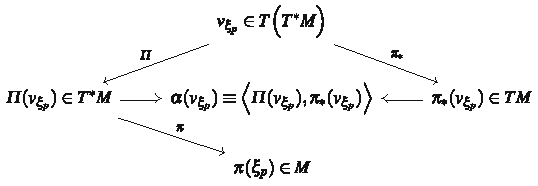
\includegraphics[width=0.744\linewidth]{images/vector/fig-B-11.pdf}
  \caption{Liouville 1-形式 $\alpha$ 用向量 $v_{\xi_p}$ 内蕴地定义. 由 $\pi(\xi_p)=p$ 定义的投影映射 $\pi:T^*M\to M$ 诱导前推映射 $\pi_*:T(T^*M)\to TM$. 映射 $\Pi$ 也是投影映射, $\Pi:T(T^*M)\to T^*M$, 由 $\Pi(v_{\xi_p})=\xi_p$ 定义. 吃掉向量 $v_{\xi_p}$ 的 Liouville 1-形式 $\alpha$ 由 1-形式 $\Pi(v_{\xi_p})$ 与向量 $\pi_*(v_{\xi_p})$ 的典范配对定义}
  \label{fig:B-11}
\end{figure}

Darboux 定理断言：如果 $(M,\omega)$ 是 $2n$ 维辛流形, 那么在每个点 $p\in M$ 的邻域 $U$ 中存在局部坐标 $(x_1,\ldots,x_n,y_1,\ldots,y_n)$, 使得辛形式 $\omega$ 可以写成
\[
\omega=\sum_{i=1}^{n}dx_i\wedge dy_i.
\]
辛几何与 Darboux 定理的一个主要应用是几何力学, 即尝试用几何术语书写经典力学. 例如, 可以把简单力学系统的 Hamiltonian 方程写成用辛形式表示的形式.

\subsection{参考文献与进一步阅读}

de Rham 上同调的两个极好导引是 Tu~\cite{ref46}, 接着是 Bott 和 Tu~\cite{ref07}. 事实上, Tu 写第一本书基本上就是为了覆盖第二本书所需的材料. 另一个参考来源, 更适合研究生和在职数学家, 是 Madsen 和 Tornhave~\cite{ref30} 的书.

辛流形与 Darboux 定理从更数学的角度由 da Silva~\cite{ref11} 覆盖, 我们在证明 Darboux 定理时特别依赖这本书. 人们可以用各种数学成熟度来逼近 Darboux 定理, 但这种方式最适合本书的目标读者. 但也可参见 Abraham、Marsden 和 Ratiu~\cite{ref01}. 此外, 任何几何力学方面的书也会覆盖辛流形的基础.

对有兴趣获得更完整处理的人来说, 几何力学有相当多有趣且良好的导引：Singer~\cite{ref39}、Holm、Schmah 和 Stoica~\cite{ref26}、Talman~\cite{ref44}、Calin 和 Chang~\cite{ref09} 以及 Holm~\cite{ref24, ref25}.

\subsection{问题}

\begin{question}\label{q:B-1}
对流形 $\mathbb{R}^n$, 证明
\[
H_{\mathrm{dR}}^k(\mathbb{R}^n)=\begin{cases}\mathbb{R}&\text{若 }k=0,\\0&\text{若 }k\geq1.\end{cases}
\]
\end{question}

\begin{question}\label{q:B-2}
求下列函数的 $df$, 
\begin{align*}
\text{(i)}\quad f=\begin{cases}7,&x\in(-\infty,0),\\-3,&x\in(0,\infty),\end{cases}\qquad
\text{(ii)}\quad f=\begin{cases}-6,&x\in(-\infty,0),\\5,&x\in(0,\infty),\end{cases} \\
\text{(iii)}\quad f=\begin{cases}\frac{14}{3},&x\in(-\infty,0),\\-6\pi,&x\in(0,\infty).\end{cases}
\end{align*}
\end{question}

\begin{question}\label{q:B-3}
解释为什么 $\mathbb{R}-\{(0)\}$ 上的每个闭 0-形式都能由两个实数精确指定, 从而 $Z^0\left(\mathbb{R}-\{(0)\}\right)\simeq\mathbb{R}^2$.
\end{question}

\begin{question}\label{q:B-4}
证明 $Z^0\left(\mathbb{R}-\{p\}-\{q\}\right)\simeq\mathbb{R}^3$, 从而 $H_{\mathrm{dR}}^0\left(\mathbb{R}-\{p\}-\{q\}\right)=\mathbb{R}^3$.
\end{question}

\begin{question}\label{q:B-5}
设 $p_1,p_2,\ldots,p_m\in\mathbb{R}$ 是互不相同的点, 并设 $M=\mathbb{R}-\{p_1\}-\{p_2\}-\cdots-\{p_m\}$. 证明 $H_{\mathrm{dR}}^0(M)=\mathbb{R}^m$.
\end{question}

\begin{question}\label{q:B-6}
论证：对具有 $m$ 个连通分量的一般流形 $M$, 有 $H_{\mathrm{dR}}^0(M)=\mathbb{R}^m$.
\end{question}

\begin{question}\label{q:B-7}
求 $k>n$ 时的 $Z^k(M)$ 与 $B^k(M)$. 证明 $H_{\mathrm{dR}}^k(M)=0$.
\end{question}

\begin{question}\label{q:B-8}
证明 $d\omega=0$.
\end{question}

\begin{question}\label{q:B-9}
用 $\tan\theta=\frac{y}{x}$ 证明当 $x\neq0$ 时 $d\theta=\omega$. 你需要回忆如何求三角函数的导数, 并使用恒等式 $\sec^2\theta=1+\tan^2\theta$.
\end{question}

\begin{question}\label{q:B-10}
用 $\cot\theta=\frac{x}{y}$ 证明当 $y\neq0$ 时 $d\theta=\omega$. 你需要回忆如何求三角函数的导数, 并使用恒等式 $\csc^2\theta=1+\cot^2\theta$.
\end{question}

\begin{question}\label{q:B-11}
用三角学论证 $\theta$ 在点 $(x,y)=(1,1)$ 处取多个值.
\end{question}

\begin{question}\label{q:B-12}
假设我们有流形 $\mathbb{R}^2-\left\{(x,0)\;\middle|\;x\leq0\right\}$, 即去掉 $x$ 轴非正部分的平面. 证明 1-形式 $\omega$ 在 $\mathbb{R}^2-\left\{(x,0)\;\middle|\;x\leq0\right\}$ 上实际上是恰当的. 类似地, 如果 $S^1$ 是单位圆, 证明在流形 $S^1-\{(-1,0)\}$ 上 1-形式 $\omega$ 是恰当的.
\end{question}

\begin{question}\label{q:B-13}
假设 $\alpha$ 是 $S^1$ 上的闭 1-形式. 定义 $r=\frac{1}{2\pi}\oint_{S^1}\alpha$. 虽然严格证明会很困难, 但给出 $\psi=\alpha-r\omega$ 是 $S^1$ 上的恰当 1-形式的合理性论证. 用它来论证 $H_{\mathrm{dR}}^1(S^1)$ 是以等价类 $[\omega]$ 为基的一维向量空间.
\end{question}

\begin{question}\label{q:B-14}
用 $n$-球的维数以及它所具有的"洞"来解释 $n$-球的 de Rham 上同调群.
\end{question}

\begin{question}\label{q:B-15}
用 2-环面的维数以及它所具有的"洞"来解释 2-环面的 de Rham 上同调群.
\end{question}

\begin{question}\label{q:B-16}
证明：对每个可能的向量 $v$ 都有 $\omega(v,w)=\sum_{i=1}^{n}(a_ib_{n+i}-a_{n+i}b_i)=0$ 意味着 $w$ 是零向量, 即 $b_1=\cdots=b_{2n}=0$.
\end{question}

\begin{question}\label{q:B-17}
用上面描述的坐标证明：Liouville 1-形式的定义 $\alpha(v_{\xi_p})\equiv\Pi(v_{\xi_p})\bigl(\pi_*(v_{\xi_p})\bigr)$ 给出公式 $\alpha=\sum_{i=1}^{n}\xi_idx_i$, 从而 $-d\alpha$ 给出典范辛形式的公式.
\end{question}
